\chapter{Geothermal Exploration with Machine Learning}\label{ch3:expl_ml_prep}

The first of the two research questions presented in Chapter \ref{ch1:intro} addressed the topic of risk in geothermal exploration. As discussed in Chapter \ref{ch2:background}, exploration has traditionally relied on geologic, geochemical, or geophysical surveys, analyzed individually or collectively through qualitative means, joint inversion methods, or play fairway analysis (PFA). Recent applications of machine-learning methods to exploration show promise in considering a range of data sources all at once, for collective insights on geothermal favorability (see Section \ref{ch2:machine_learning}). This chapter describes a methodology for applying machine learning and uncertainty analysis to the study area in Southwestern New Mexico introduced in Section \ref{ch2:case_outline}, as an investigation in data-driven risk-mitigation for geothermal exploration.

\section{Data Sources}\label{ch3:expl_data_src}

This investigation brings together a total of twenty-five (25) data sets covering the Southwestern NM study area (Table \ref{tab:features}). Data were collected from previously published works, open-access databases, or derived from those original sources as secondary products. The form of the data varies between pre-gridded raster files, point data sets with repeat or overlapping measurements, non-overlapping point sets, and line data. Previous research efforts produced the raster files or raster-ready gridded data that comprise ten of the data sets (also called ``features”). Three features are generated by running procedures on one of the existing rasters. The remaining layers were created from polylines (5), overlapping points (4), and non-overlapping points (3). Although complex interactions between earth systems should be expected, these layers represent the ``independent'' or \textit{predictor} variables for analysis purposes. Section \ref{ch3:feat_corr} explains how evaluating collinearities between features allows for pre-screening before modeling, and further analysis of feature importances in Chapter \ref{ch5:ml_results} helps hone in on the most influential features for simpler prediction models.

\begin{table}
\centering
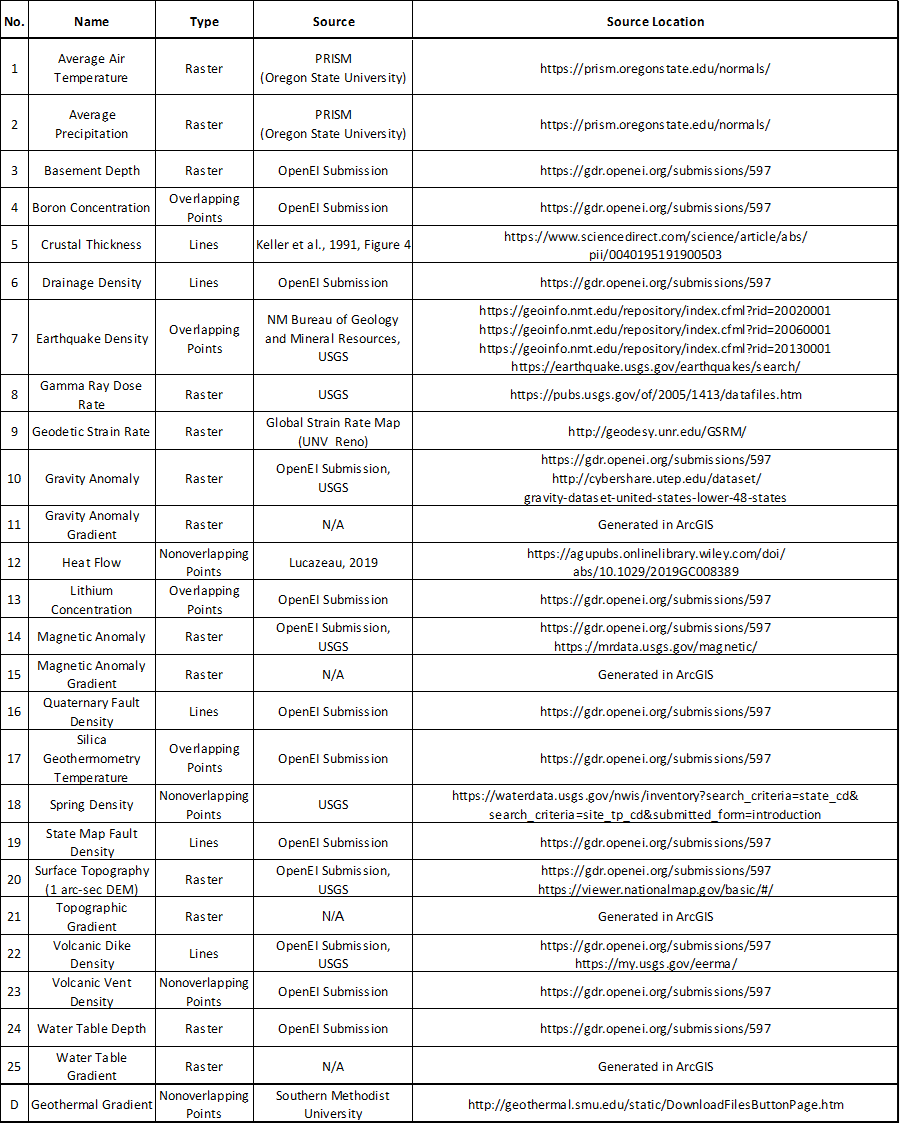
\includegraphics[width=\textwidth]{Table-Features.png}
\caption[Southwestern New Mexico feature list]{List of data sets included in this analysis. Data type, source, and source location are noted. Suggested feature-sensitive risk elements include fluids (F), heat/temperature (T), and structure/permeability (P). Numbered features are treated as predictor variables. `D' indicates the dependent or response variable. See Appendix \ref{app:A_data_layers} for details on how each feature GIS layer was constructed for modeling.}
\label{tab:features}
\end{table}

As discussed in Section \ref{ch2:sysfund}, viable geothermal systems require permeability, heat, fluids, seal, and recharge. Following the more simplified PFA risk elements of \citet{bielicki_hydrogeolgic_2015}, an explorationist will want to first identify where fluids, heat, and permeability together define a favorable setting, then consider seal as a final screening factor. The chosen feature inputs collectively address the first three elements, as noted in Table \ref{tab:features}. Rather than defining a ``dependent'' or \textit{response} variable that describes a total favorability score, this thesis focuses on a proof-of-concept predictive workflow for a physically-measurable quantity associated with the heat risk element: geothermal gradient. This choice was made because a) a combined favorability score is less straight-forward to define and calibrate than geothermal gradient, b) gradient point data is available from suitable compilations of well measurements covering the study area, c) geothermal gradient provides a direct proxy for accessible heat content, and d) for EGS applications, the crucial element that must be naturally present is heat. Heat flow might be a reasonable alternative response variable, however heat flow values in the available well database were derived from geothermal gradient and hence are not primary source data. Another alternative could be geothermometer measurements (see Section \ref{ch2:geologic_data}) that characterize reservoir temperature, but the uncertainty in fluid pathways leading to the measurement location means these values suffer from less spatial and depth certainty than geothermal gradient.

Regarding the remaining risk elements, permeability, fluids, and seal could all be separately predicted using the methods described in this study. A final favorability score would then need to be derived from the combined risk element maps as is done in PFA risk assessments. This extended methodology is outside the scope of this thesis and thus appears in the list of future work opportunities in Chapter \ref{ch9:future_work}.

\section{Data Preparation}\label{ch3:data_prep}
Before experimenting with a variety of machine learning methods, all input data sets must first be transformed into fully-complete \acrlong{gis} (\acrshort{gis}) layers such that any location within the study area has a corresponding set of predictor values. Steps taken to condition and process each layer are introduced in this chapter and detailed in Appendix \ref{app:A_data_layers}. The following section reviews several fundamental concepts and algorithms utilized in the preparation of the data layers.

\subsection{Fundamentals}\label{ch3:data_prep_fundamentals}
\subsubsection{Extents}\label{ch3:extents}
The data sets imported into ArcGIS and Python scripts for feature preparation required cropping, gridding, or, less frequently, extrapolation to match each other in coverage of the Southwestern New Mexico study area. Two polygons were used for this purpose:

\begin{itemize}
\item \textbf{Regional Polygon}: this is a simple rectangular polygon capturing the broader Southwestern NM region, defined by the following corner points in $^\circ$N Latitude and $^\circ$E Longitude: \\ (-31.3, -109.1), (31.3, -105.9), (35.4, -105.9), (31.3, -109.1)
\item \textbf{\acrlong{aoi} (\acrshort{aoi})}: this polygon appears in most map figures in this thesis (e.g., Figure \ref{fig:meshgrid}) and is the perimeter of a nine-county block in Southwest New Mexico that includes Cibola, Valencia, Catron, Socorro, Grant, Sierra, Luna, Dona Ana, and Hidalgo counties.
\end{itemize}

\subsubsection{Point Mesh Grid}
\label{ch3:meshgrid}
Machine learning models generally treat data as a matrix of observations. The concept of a geospatial dataframe follows this paradigm, where each row represents a discrete location specified in latitude and longitude columns, and all other columns contain feature values for that location. Since the area outlined by the study AOI covers 97,469 km$^2$, and each location is described by 25 features and 2 map coordinates, the matrix of the study area at 1 km$^2$ resolution would be over 2.6 million values in size. This could be problematic since the time complexity of some machine learning methods shows non-linear growth with data size, e.g., decision trees (Section \ref{ch3:decision_trees}) have $O(\text{m} \cdot \text{n} \cdot \log_2(\text{n}))$ complexity, where n is the number of observations and m is the number of features \citep{sani_computational_2018}. As such, a coarser resolution of $0.025^\circ$ ($\approx$2.5 km on average across the AOI) was selected as a manageable sampling interval for this study. To support downsampling operations, the ArcGIS \textit{Create Fishnet} tool was used to generate a $0.025^\circ$ x $0.025^\circ$ mesh grid that, when constrained to the AOI polygon, consists of 15,137 point locations (Figure \ref{fig:meshgrid}). Data preparation steps use this mesh grid point set where noted in Appendix \ref{app:A_data_layers}, and final model predictions are made on these points to enable direct comparison between different model results. 

\begin{figure}
\centering
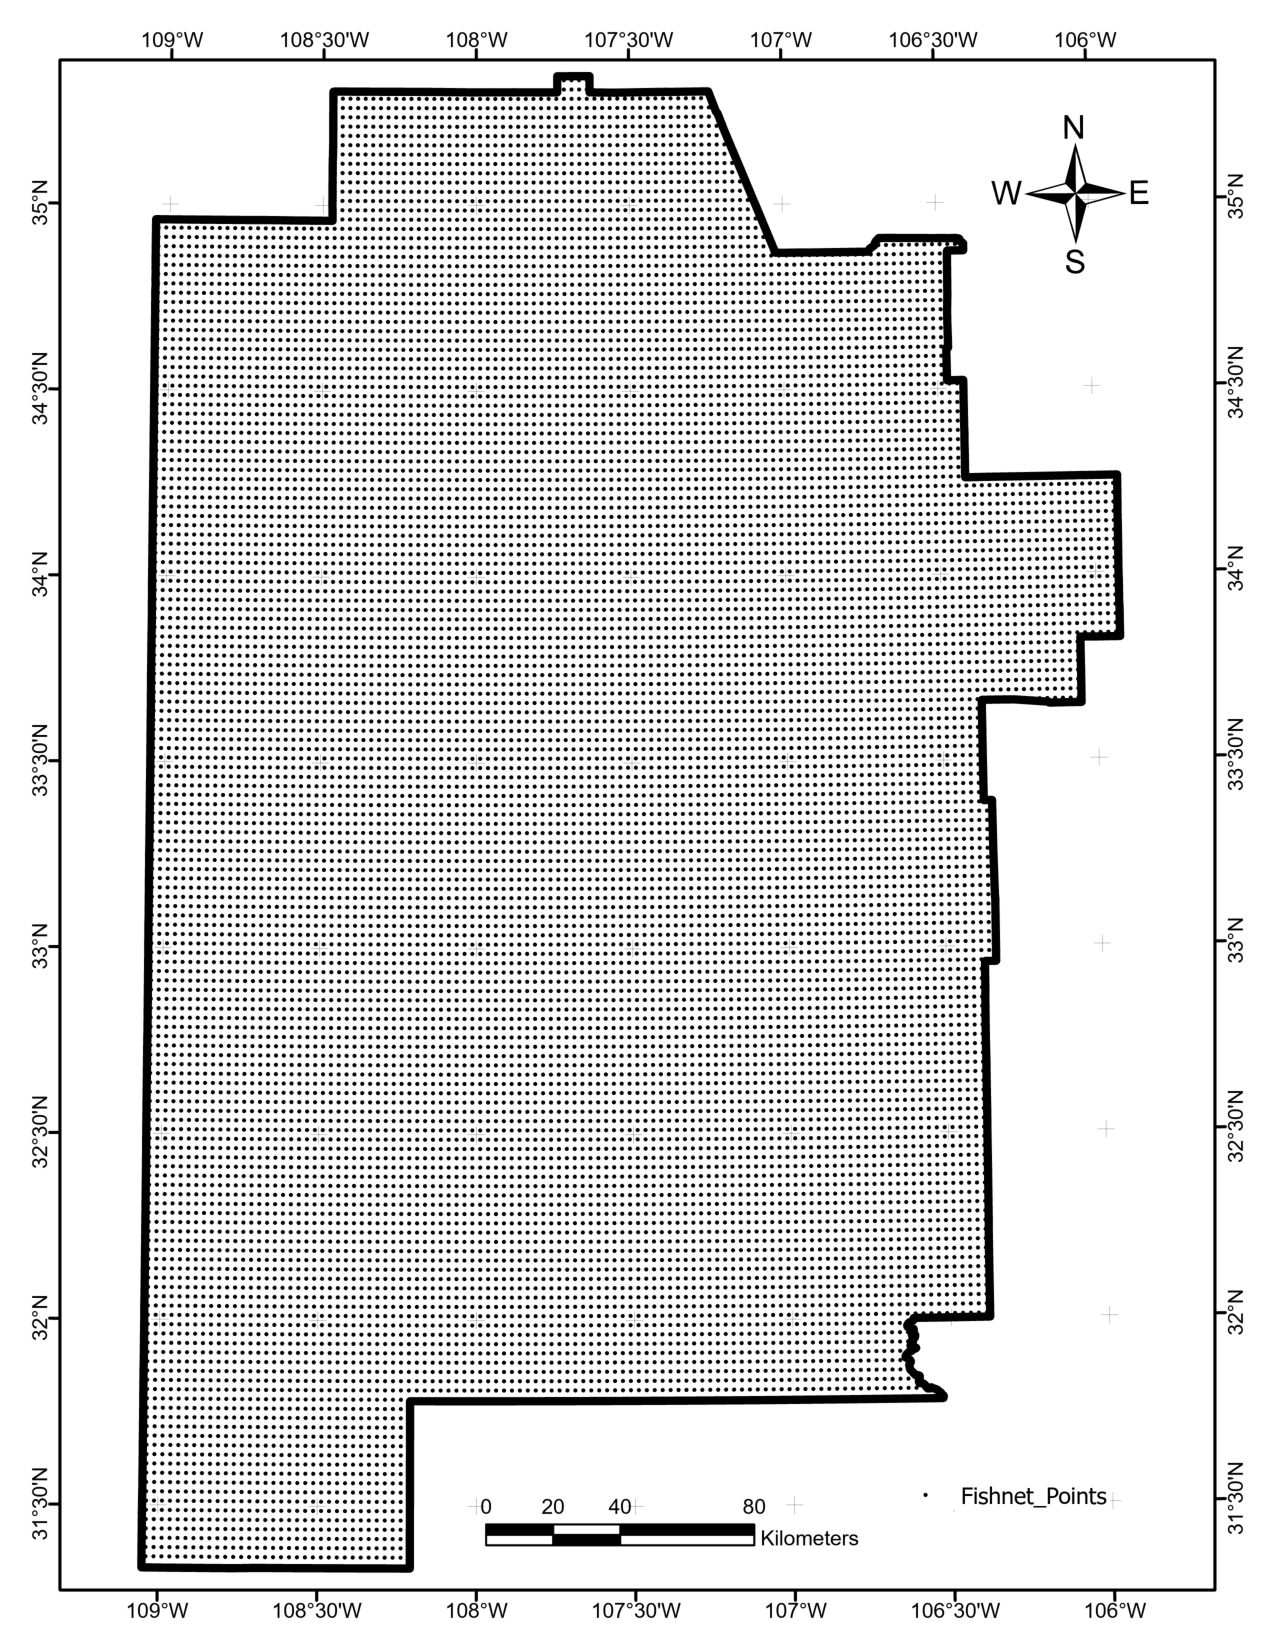
\includegraphics[width=0.75\linewidth]{templates/images/Figure-Fishnet.pdf}
\caption[Mesh grid point set]{Mesh grid of points spaced $0.025^\circ$ apart in latitude and longitude. The mesh grid point set is used for data preparation and model predictions.} 
\label{fig:meshgrid}
\end{figure}

\subsubsection{Density Estimation}\label{ch3:density_est}
One technique for converting a discrete set of points into a continuous field of values uses the concept of point density. The \acrlong{kde} (\acrshort{kde}) method fits a smooth function (kernel) to each point with the constraint that the volume under a kernel surface is 1.0. Density values assigned to cells of a gridded surface or raster image represent the sum over the kernels crossing those cells. The kernel density tool can provide an estimate of density anywhere within the AOI, but it requires a kernel radius that sets the distance over which a point influences the density value. If left undefined, ArcGIS defaults to an optimal radius value based on a bandwidth formula \citep{esri_kernel_2021}. ArcGIS uses Silverman quartic kernel as the functional basis in the \textit{Kernel Density} operation \citep{esri_kernel_2021,silverman_density_1986}.

Polyline data can also be fit with smoothly-curved surfaces using the density concept. The maximum value of the elongate surface follows the trace of the polyline, and the surfaces decays in value away from the line over a distance determined by the radius, which defaults to the bandwidth estimate. The volume under the surface scales with line length. For more details on the ArcGIS implementation of polyline density estimation, refer to the \textit{Density toolset} documentation on \textit{Kernel Density} \citep{esri_kernel_2021}.

\subsubsection{Surface Fitting}\label{ch3:surface_fit}
A multitude of algorithms exist for the purpose of fitting a set of values with a surface, thereby providing a means for interpolating missing values. Methods used in this thesis include the following four operations:

\begin{itemize}
\item{\textbf{Splines}}\label{ch3:splines} - Spline functions have a well-defined mathematical formulation that minimizes curvature while exactly fitting the input points. Regularized splines add a third derivative term, controlled by a weight parameter, that enforces a higher degree of smoothness with the trade-off of some data misfit. This is helpful if outliers in the input point set would otherwise distort the spline fit. For details on the ArcGIS implementation for splines, refer to the \textit{Interpolation toolset} documentation on the \textit{Spline} function \citep{esri_spline_2021}.
\item{\textbf{Topo to Raster}}\label{ch3:topo2r} - The ArcGIS \textit{Topo to Raster} operation creates surfaces that honor the input data, typically contour sets, while ensuring i) correct representation of abrupt morphological features like rivers and ridges and ii) connectedness of drainage patterns. Specifically, \textit{Topo to Raster} uses an iterative finite difference method and an algorithm to remove sink points not supported by the input data, assuming natural sinks are rare and erroneous features in an interpolated surface. For details on the ArcGIS implementation, refer to the \textit{Interpolation toolset} documentation on the \textit{Topo to Raster} function \citep{esri_topo_2021}.
\item{\textbf{Ordinary Kriging}}\label{ch3:kriging} - Kriging methods are geostatistical algorithms that take the correlation distance and directional bias into account when creating a surface. The two tasks involved in kriging include first estimating the functions that characterize these spatial relationships, then using these functions to generate predictions for interpolation (or extrapolation). For the first task, semivariograms are calculated by binning the semivariance of points based their distance from each other, then fitting a model curve (e.g., linear, spherical, exponential) to these values. Semivariograms can be anisotropic, meaning they vary with direction. The second task uses the semivariogram to define a weighted average of the input data when estimating new values. For more details on the ArcGIS implementation of kriging operations, refer to the \textit{Interpolation toolset} documentation on the \textit{Kriging} function \citep{esri_kriging_2021}.
\item{\textbf{\acrlong{ebk} (\acrshort{ebk})}}\label{ch3:ebk} - The EBK algorithm extends ordinary kriging by automating parameter selections and accounting for uncertainty in semivariogram estimation. Ordinary kriging generates a single variogram and treats it as ground truth while EBK generates an ensemble of semivariograms that can more accurately estimate standard errors. As a computationally heavy method, EBK takes much longer to apply than other curve-fitting operations. For more details on the ArcGIS implementation of EBK, refer to the documentation on the \textit{Empirical Bayes Kriging} function \citep{esri_empirical_2021}.
\end{itemize}

\subsection{Data Conditioning}\label{ch3:conditioning}

%\begin{wrapfigure}{R}{0.35\linewidth}
\begin{figure}
\centering
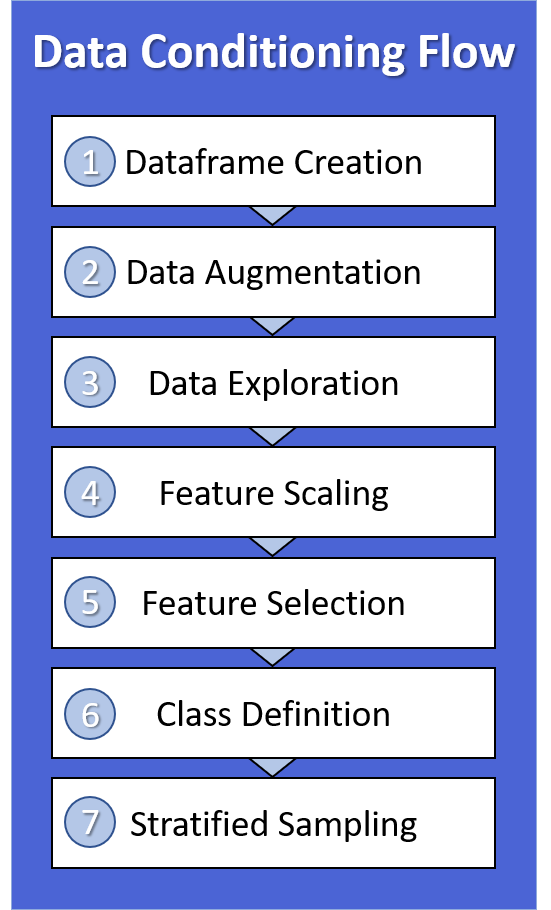
\includegraphics[width=0.35\linewidth]{templates/images/Flow-DataConditioning.png}
\singlespacing
\caption[Data conditioning workflow]{Workflow for conditioning data prior to predictive modeling.}
\label{fig:DC_Flow}
%\end{wrapfigure}
\end{figure}
After building the various GIS data layers, several data conditioning steps were taken to explore variable relationships, rationalize feature choices, and prepare data values for modeling. Figure \ref{fig:DC_Flow} outlines the general workflow followed, detailed more extensively below.

\subsubsection{Dataframe Creation}
Feature GIS maps spanning the full AOI provide the primary data resource, but predictions of geothermal gradient require ground truth observations for training a predictive model. Initially, two separate data sets could be constructed for further evaluation. The first is a \acrlong{fds} (\acrshort{fds}) that consists of feature values extracted using the pre-defined point mesh grid (Figure \ref{fig:meshgrid}), resulting in 15,137 records for the 25 predictors. This data set does not include values for the response variable. Although there is a geothermal gradient feature layer described in Section \ref{app:dl_geothermal_gradient}, this is just a derived layer for comparison and not ground truth. The second data set was built from actual geothermal gradient observations in the SMU database described in Section \ref{app:dl_geothermal_gradient}, combined with 25 feature values extracted from the GIS maps at the observation locations. This data set is hereafter referred to as \acrlong{wds} (\acrshort{wds}). Both FDS and WDS were stored in ``geodataframes'' consisting of the feature values and their associated latitude and longitude coordinates. These structured matrices are compatible with machine learning techniques like those found in the scikit-learn \citep{pedregosa_scikit-learn_2011} and TensorFlow \citep{abadi_tensorflow_2016} Python packages. 

\subsubsection{Data Augmentation}\label{ch3:augmentation}
\begin{figure}
%\begin{wrapfigure}{R}{0.5\linewidth}
\centering
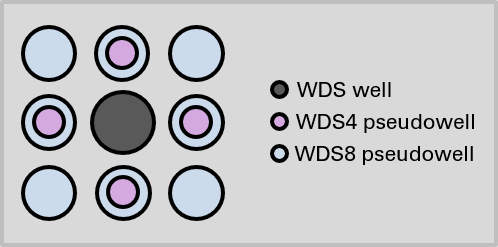
\includegraphics[scale=0.9]{templates/images/Figure-AugmentedWells.png}
\singlespacing
\caption[Data augmentation strategy]{The data augmentation strategy creates neighboring well locations around each original well in the WDS (dark gray). For WDS4, pseudowells (purple) are placed to the N, S, E, and W. For WDS8, pseudowells (blue) are placed at eight locations around the central well. Latitude and longitude offsets are $\pm0.01^\circ$ for pseudowell placement.}
\label{fig:data_augmentation}
%\end{wrapfigure}
\end{figure}

Noting the AOI under investigation spans over 97,000 km$^2$, the relatively small size of WDS ($\approx$600 observations) raises concern over whether enough data is available to obtain data-driven insights using supervised learning methods. If predictions are reduced to just locations in the AOI mesh grid, there are still 2 orders of magnitude difference between ground truth observations and the points being predicted, exacerbated further by the need to partition the input data into one subset for training and two others for model validation and testing as a machine learning best practice \citep[e.g.,][p.\ 222]{hastie_elements_2009} (see Section \ref{ch3:strat_sample}). 

Data augmentation methods boost the size of a sparse data set by using basic assumptions or heuristics to create additional data points. This study applies the concept of spatial autocorrelation at the heart of variography and kriging methods; in geography, all things are related, but the correlation increases as the spatial distance decreases \citep[Chapter\ 13]{gimond_intro_2021}. For each well location in the WDS, an additional four points were placed to the north, south, east, and west by adding or subtracting a constant 0.01$^\circ$ to each well’s geographic coordinates (Figure \ref{fig:data_augmentation}). Feature values were extracted from the layer maps in ArcGIS at these ``pseudowell'' locations. For the response variable, geothermal gradient, an interpolation layer was created from the WDS observations using the ArcGIS \textit{Kriging} function with spherical variogram, auto-determined lag size of 0.097, and variable search radius with 12-point requirement. Gradient values were extracted from this layer for each pseudowell. The use of an interpolated gradient layer avoided conflict in pseudowell values for close-proximity real well locations since step-out pseudowells for neighboring original wells could (and do) overlap. This overall workflow generated a new data set with 2,995 observations within the study AOI, referred to as \acrshort{wds4}. 

Extending this method further, a second augmented data set placed pseudowells to the NE, SE, NW, and SW as well, resulting in eight pseudowells for every original well in the WDS (Figure \ref{fig:data_augmentation}). Restricting the results to the AOI, this produced a data set with 5,386 observations (\acrshort{wds8}) for use in training and testing of machine learning models.

\subsubsection{Data Exploration}
The comprehensive coverage of FDS makes it an appealing data set to use for exploring the attributes and relationships of the 25 data layers. Although care was taken to ensure each GIS layer fully spanned the AOI, a search for missing values identified 163 \acrshort{nan}s (i.e., \acrlong{nan}, unassigned values) among the features. The corresponding data rows plot along the study area boundary and likely represent places where one or more data layers ended just short of the point locations in the AOI mesh grid. These rows were dropped from FDS, reducing its size to 15,007 records.

Histograms can offer insights on the data distributions of predictor variables. Based on Figure \ref{fig:unscaled_hists}, only the magnetic anomaly layer has the appearance of a zero-mean Gaussian distribution. All other variables are offset and skewed to some extent. Many statistical tools rely on the assumption of normally-distributed random variables, so skewness can be problematic for modeling \citep[p.\ 85]{montgomery_statistical_2012}. These results suggest variable scaling and transformations will be a useful part of data preparation \citep[p.\ 221]{montgomery_statistical_2012}. 

\begin{figure}[!htp]
\centering
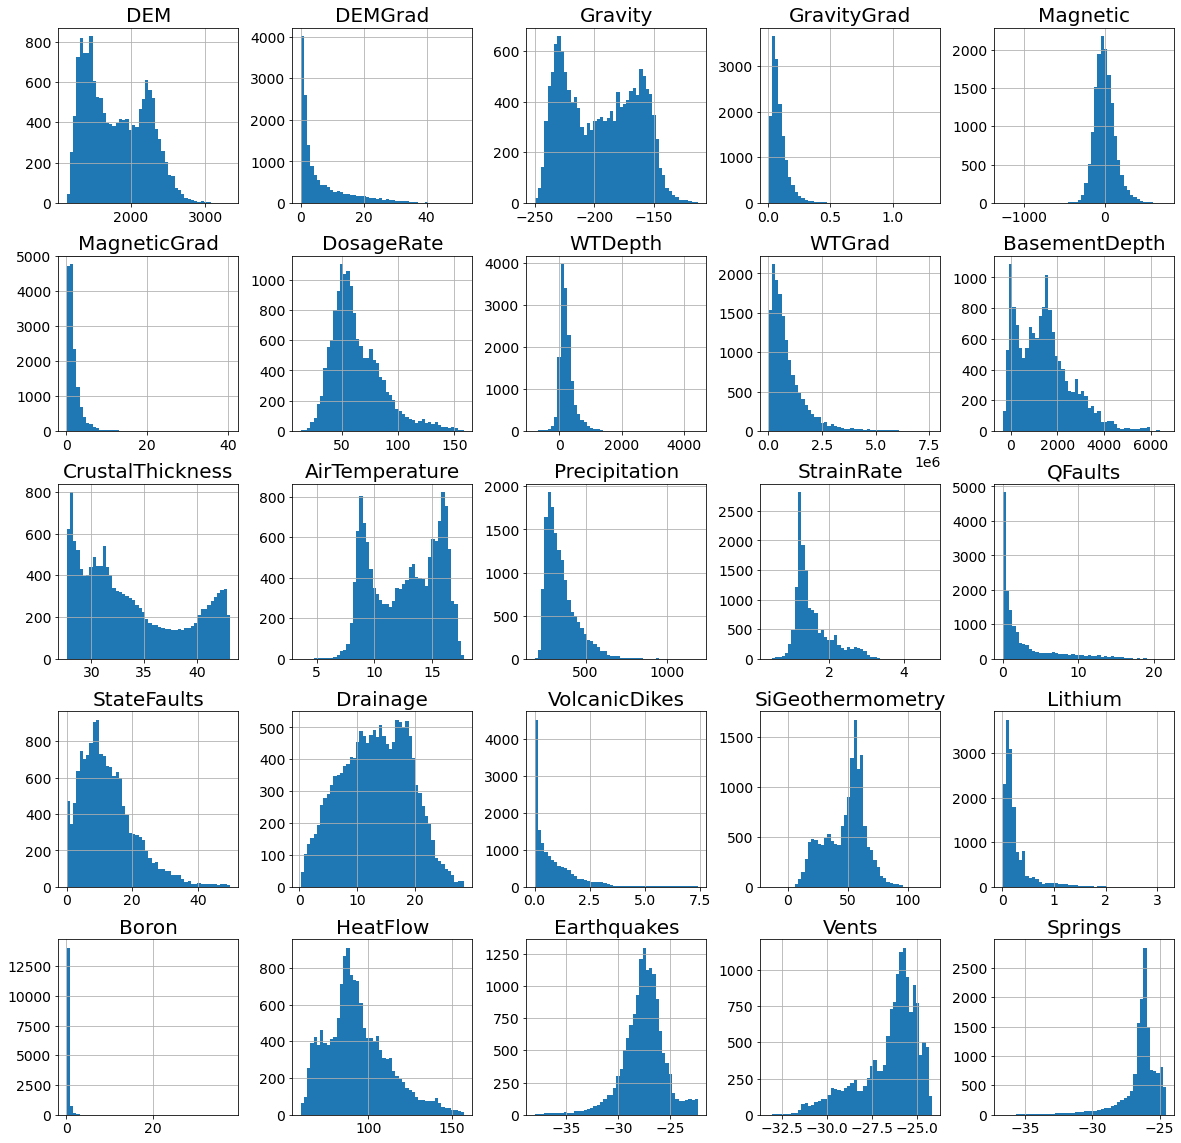
\includegraphics[width=\textwidth]{templates/images/Figure-Unscaled_Histograms.png}
\caption[Unconditioned FDS histograms]{Histograms of the 25 features using 50 bins and FDS data. No scaling or transformations were applied to the data.}
\label{fig:unscaled_hists}
\end{figure}

Scatter plots between variables can highlight collinear behavior where a close relationship between two predictors creates uncertainty in their balance, that is, their individual contributions to the response variable \citep[p.\ 99]{james_introduction_2013}. This can reduce the accuracy of model parameters like regression coefficients, impact the statistical significance of predictors, and lead to overly complex models \citep[p.\ 100-101]{james_introduction_2013}. Figure \ref{fig:unscaled_scatter} illustrates all permutations of feature pairwise relationships. Although individual plots are too small to appreciate in detail, the overall shapes of the plots suggests some linear behavior between a handful of variables. The inset maps illustrate two examples of collinearity, and the third shows how skewness in variable distributions makes it difficult to discern some feature relationships.

\begin{figure}[!htp]
\centering
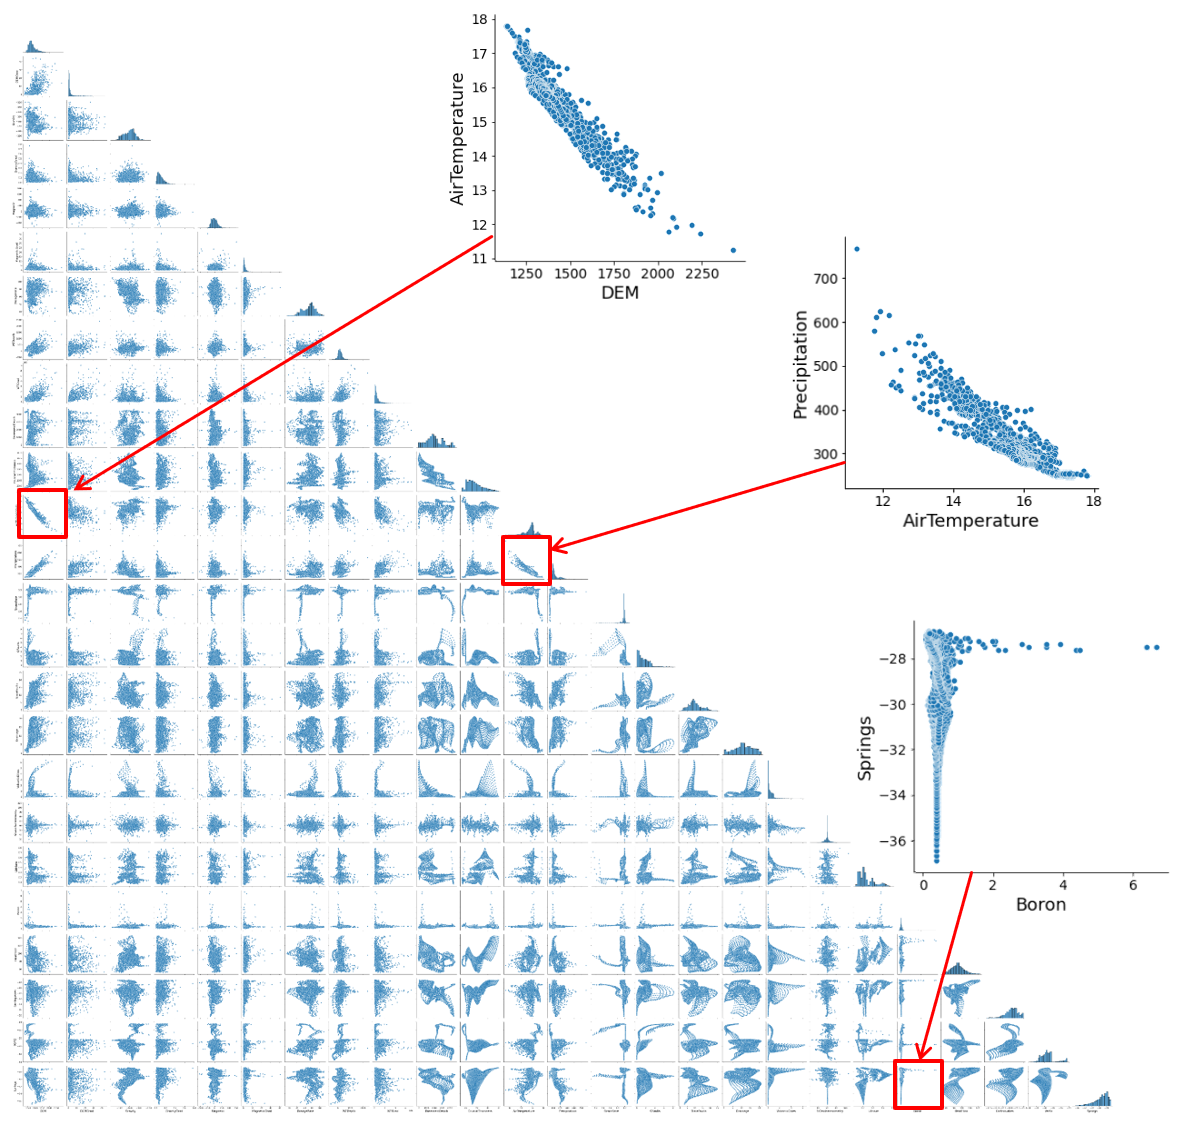
\includegraphics[width=\textwidth]{templates/images/Figure-Scatterplot_Unscaled_Features.png}
\caption[Unscaled FDS scatter plots]{Scatter plots between all possible pairs of the 25 features. The upper two plot call-outs illustrate collinear relationships. The lowermost highlighted plot shows the impact of skewed distributions. Note the difference in axis ranges depending on the variable. All plots show the first 2,000 points of the 15,007-point FDS.}
\label{fig:unscaled_scatter}
\end{figure}

\subsubsection{Feature Scaling}\label{ch3:scaling}
Large differences in the ranges and average values of the predictor variables are also evident in the scatter plots in Figure \ref{fig:unscaled_scatter}. For some machine learning algorithms, variables with larger value ranges can have an out-sized effect on the model, so scaling variables to comparable ranges and removing variable bias is an important step in data conditioning. Scaling also makes a predictor closer to the standard normal in appearance, i.e., $N(\mu=0, \sigma=1)$, as implicitly required by some statistical methods. The scikit-learn \textit{StandardScalar} function transforms data using the Z-score formulation \citep{scikit-learn_sklearnpreprocessingstandardscaler_2021}:

\begin{equation}
    Z = \frac{(x - \mu)}{\sigma}
\end{equation}

This data scaling can be directly paired with non-linear data transformations that alter the shape of variable distributions, replacing skewness with more Gaussian-like symmetry. One such transformation is the Yeo-Johnson method, which can handle both positive and negative data. The Yeo-Johnson power transformation actually represents a family of transformations, the choice of which depends on a single parameter, $\lambda$ \citep{yeo_new_2000}:

\begin{equation}
    x_i^{(\lambda)} = 
    \begin{cases}
      [(x_i + 1)^{\lambda)}-1]/\lambda & \text{if $\lambda \neq 0$, $x_i \geq 0$,}\\
      \ln{(x_i + 1)} & \text{if $\lambda = 0$, $x_i \geq 0$,}\\
      -[(-x_i + 1)^{2-\lambda}-1]/(2-\lambda) & \text{if $\lambda \neq 2$, $x_i < 0$,}\\
      -\ln{(-x_i + 1)} & \text{if $\lambda = 2$, $x_i < 0$}
    \end{cases}  
\end{equation}

Scikit-learn supports Yeo-Johnson through the \textit{PowerTransformer} preprocessing tool that automatically estimates the $\lambda$ parameter using maximum likelihood \citep{scikit-learn_sklearnpreprocessingpowertransformer_2021}. Figure \ref{fig:scaled_hist} shows the same histograms after applying both standard scaling and Yeo-Johnson transformation to the predictor variables. Many of the distributions appear much less skewed, and all have zero-mean and unit variance.

\begin{figure}[!htp]
\centering
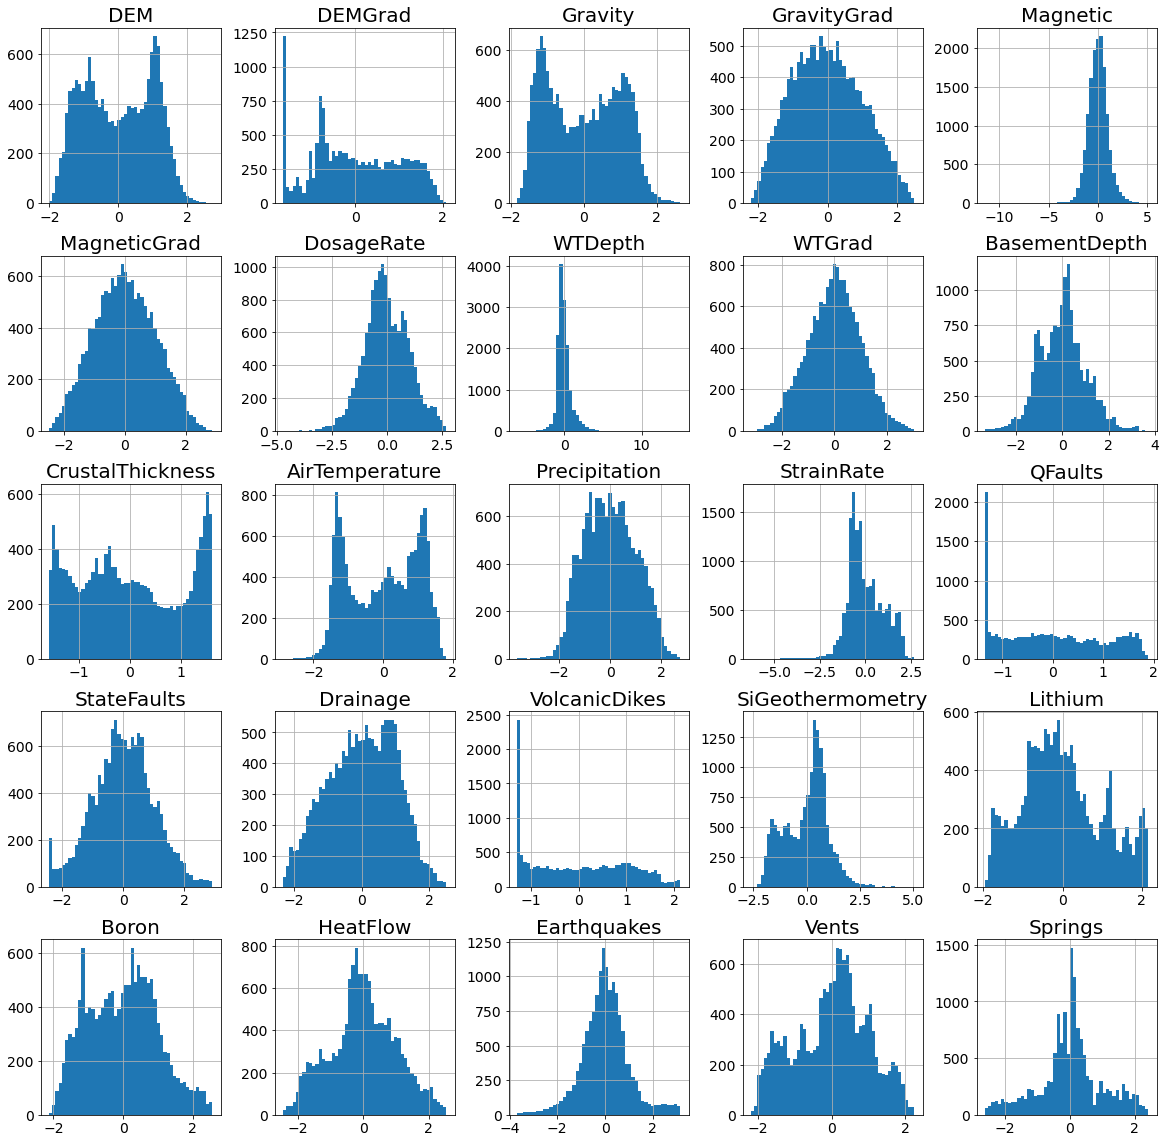
\includegraphics[width=\textwidth]{templates/images/Figure-Scaled_Histograms.png}
\caption[Conditioned FDS histograms]{Histograms of the 25 features after standard-scaling and Yeo-Johnson transformation of FDS. Plots use 50 bins.}
\label{fig:scaled_hist}
\end{figure}

Scaling and transformation also impact the variable pairwise scatter plots. Figure \ref{fig:scaled_scatter} illustrates the improvement in scatter plot appearances as a result of the feature conditioning. With greater spread in the variable distributions, relationships are more readily apparent.

\begin{figure}[!htp]
\centering
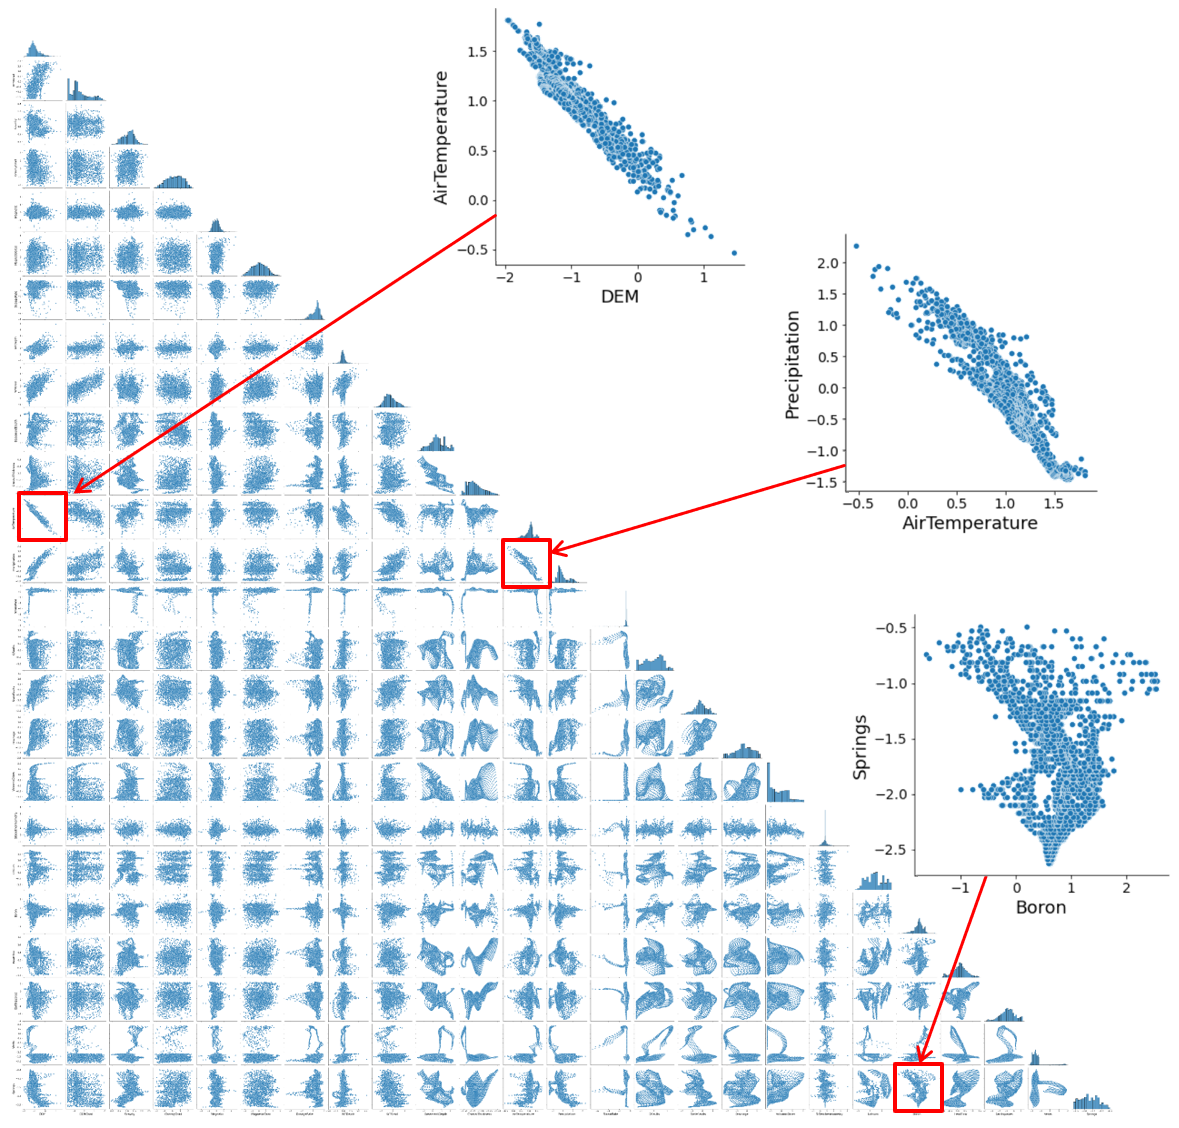
\includegraphics[width=\textwidth]{templates/images/Figure-Scatterplot_Scaled_Features.png}
\caption[Scaled FDS scatter plots]{Scatter plots between all possible pairs of the 25 features after standard scaling and Yeo-Johnson transformation for FDS. The upper two plot call-outs illustrate collinear relationships. The lowermost highlighted plot shows the impact of Yeo-Johnson transformation on revealing variable relationships that were hidden by skewed distributions. All plots show the first 2,000 points of the 15,007-point FDS.}
\label{fig:scaled_scatter}
\end{figure}

\subsubsection{Feature Correlation}\label{ch3:feat_corr}
Another way to evaluate collinearity between two features is to calculate their correlation coefficient. The standard Pearson correlation coefficient ($r$) is strictly defined as the covariance between two variables, scaled by the product of their standard deviations. On a per-sample basis, this becomes \citep[p.\ 70]{james_introduction_2013}:

\begin{equation}
    r = \frac{\Sigma(x_i-\bar{x})(y_i-\bar{y})}{\sqrt{\Sigma{(x_i-\bar{x})^2} \Sigma{(y_i-\bar{y})^2}}}
\end{equation}

When $r$ is close to zero, no measurable covariance takes place between the two variables. Values close to 1 or -1 suggest the two variables are linearly-related, where the sign indicates direction of the relationship. A lower triangular matrix of pairwise correlation coefficients was calculated using the scaled, transformed version of FDS (Figure \ref{fig:corr_matrix}). Average Air Temperature stands out as highly collinear with multiple variables: DEM (-0.97), Gravity Anomaly (0.89), and Crustal Thickness (-0.89). Crustal Thickness also shows some collinearity with Gravity Anomaly (-0.88) and DEM (0.80). The same is true for Gravity and DEM (-0.83).

\begin{figure}[!htp]
\centering
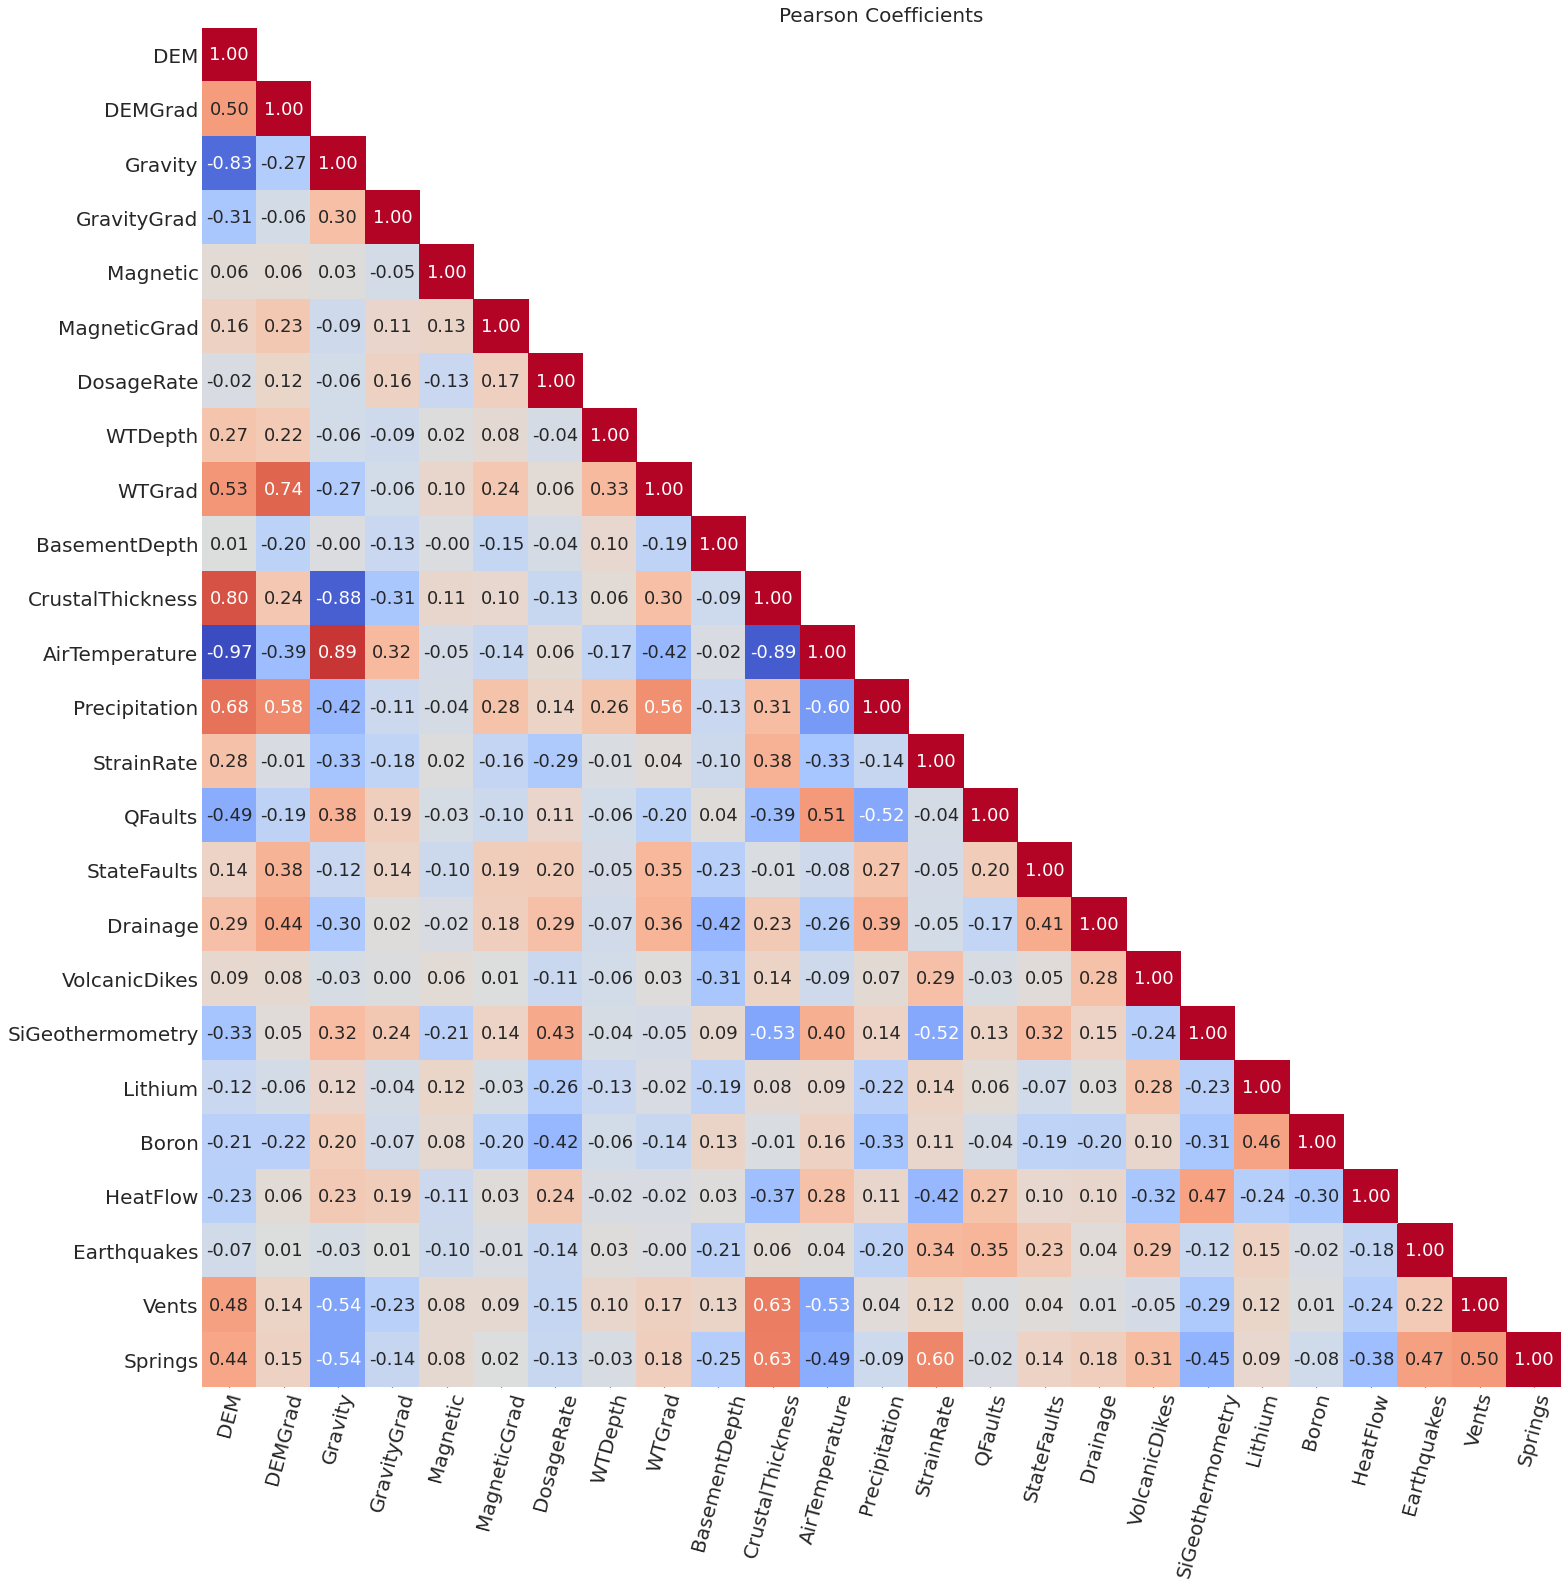
\includegraphics[width=\textwidth]{templates/images/Figure-Scaled_Correlation_Matrix.png}
\caption[Feature correlation matrix]{Correlation matrix with Pearson correlation scores for each feature pair based on the scaled and transformed version of the FDS.}
\label{fig:corr_matrix}
\end{figure}

Focusing on the related Earth systems, the logic behind these relationships makes sense. High surface elevations recorded in the DEM layer will have correspondingly lower average air temperatures, hence snow caps appearing on mountains. In addition, if the crust is assumed to be in isostatic equilibrium with the mantle --- like an iceberg floating in the ocean --- topographic highs will be supported by thick roots and DEM will directly covary with crustal thickness. And since crustal densities are less than those of the underlying mantle, displacement of upper mantle by crustal roots (high crustal thickness) results in a lower average density and negative gravity anomaly values. The reverse is true as well; thinner crust will correspondingly tie to positive gravity anomaly values.  

Of these variables, only Air Temperature and DEM have a correlation value over 0.9. In fact, a 0.97 $r$-value suggests Air Temperature and DEM are nearly interchangeable in the value of information they provide to a predictive model. Since air temperature does not directly relate to subsurface characteristics except for thermal conditions at zero-depth, Average Air Temperature can be removed from the main set of predictors to reduce overall collinearity in the data set. Crustal Thickness and Gravity Anomaly both similarly show non-ideal $r$-values, but feature ranking while modeling will provide another opportunity to consider which of them might need to be removed (e.g., Section \ref{ch3:xgb_shapley}).

\subsubsection{Classification Framework}\label{ch3:gradient_classes}
Geothermal gradient can be treated as a continuous variable and predicted directly using regression methods. Alternatively, binning the geothermal gradient into discrete ranges changes the approach into a classification problem. In the context of exploration, geospatial classifications have a direct corollary in the typical traffic-light coloration of PFA favorability maps and other simplified displays of complex risk. Furthermore, regression model results provide exact geothermal gradient estimates, which could easily be mistaken for certainty in a largely under-constrained problem. The binning approach is adopted in this thesis largely based on previously published work.

\begin{wraptable}{R}{0.4\linewidth}
\centering
\begin{tabular}{|c|c|}
\hline
\textbf{Gradient Range} & \textbf{Class} \\ \hline
{[}\;0 K/km, 30 K/km)     & 0                    \\ \hline
{[}\;30 K/km, 40 K/km)    & 1                    \\ \hline
{[}\;40 K/km, 60 K/km)    & 2                    \\ \hline
{[}\;60 K/km, 999 K/km)   & 3                    \\ \hline
\end{tabular}
\singlespacing
\caption[Geothermal gradient classes]{Geothermal gradient ranges and assigned class values using set notation. Ranges are left-inclusive.}
\label{tab:geothermal_gradient_classes}
\end{wraptable}

The \textit{Geothermal Gradient Map of the Conterminous United States} published in 1991 separates geothermal gradient into five 15 K/km bins that cap out with 60-75+ K/km \citep{lanl_geothermal_1991}. \citet{armstead_heat_1987} instead defined non-thermal gradients as 20-25 K/km, thermal gradients as $\geq$38 K/km, and hydrothermal gradients as 60-80 K/km on average. \citet{tester_economic_1990} reframed this model with discrete representative values for three EGS grades: high = 80 K/km, mid = 50 K/km, and low = 30 K/km. In a later iteration, \citet{herzog_economic_1997} confirmed ranges for EGS resources: high-grade for >60 K/km, mid-grade for 40-60 K/km, and low-grade for <40 K/km. This thesis extends the Herzog model by adding a non-thermal range as <30 K/km, recognizing the average geothermal gradient ranges from 25-30 K/km and anything below that would be ill-suited for geothermal exploration and development (see Table \ref{tab:geothermal_gradient_classes}).

Preparation of well data sets WDS, WDS4, and WDS8 first involved removing records with NaN values or negative geothermal gradients. The remaining records were split into the gradient categories defined in Table \ref{tab:geothermal_gradient_classes}. Distributions of class values for all data sets are shown in Table \ref{tab:data_set_class_count}. For FDS, the class break-down is based on the extrapolated \citet{bielicki_hydrogeolgic_2015} geothermal gradient layer (Figure \ref{fig:feat_pfa_geotherm_gradient}) sampled using the AOI mesh grid (Figure \ref{fig:meshgrid}). Note that class imbalance exists in all data sets; mid-grade values dominate in the FDS, but the well data sets show a bias toward high-grade examples with few non-thermal examples. This is a common conundrum when using well data for characterization and analysis; drilling campaigns tend to target areas to drill based on chance of success rather than drilling at random, so low-side under-representation tends to be ubiquitous.  
\\
\begin{table}[htp]
\centering
\begin{tabular}{c|c|c|c|c|}
\cline{2-5}
 & \textbf{FDS} & \textbf{WDS} & \textbf{WDS4} & \textbf{WDS8} \\ \hline
\multicolumn{1}{|c|}{\textbf{Class 0}} & 2,394 & 20 & 101 & 184 \\ \hline
\multicolumn{1}{|c|}{\textbf{Class 1}} & 4,432 & 99 & 499 & 905 \\ \hline
\multicolumn{1}{|c|}{\textbf{Class 2}} & 6,243 & 232 & 1,144 & 2,029 \\ \hline
\multicolumn{1}{|c|}{\textbf{Class 3}} & 1,938 & 245 & 1,229 & 2,226 \\ \hline
\multicolumn{1}{|c|}{\textbf{Total}} & 15,007 & 596 & 2,973 & 5,344 \\ \hline
\end{tabular}
\caption[Data set class distribution]{Distribution of geothermal gradient classes for each data set.}
\label{tab:data_set_class_count}
\end{table}

\subsubsection{Stratified Sampling}\label{ch3:strat_sample}
Supervised machine learning methods tune model predictions based on the input data provided during training. In approximating the target function, i.e., the response variable, these models seek to minimize an objective function as much as possible. The pitfall here lies in the representativeness of the training data set; if a model exactly matches the input data, it may not generalize well to other unseen observations. This would be a high variance model, meaning the model predictions are strongly coupled to the characteristics of the training data. Variance trades off with model bias, which includes simplifying assumptions on the form of the target function. The bias-variance trade-off is a core concept in machine learning \citep[p.\ 33-36]{james_introduction_2013} and drives many of the model decisions made within this thesis.

One method of reining in the high variance overfitting problem involves splitting the input data set into training and testing subsets. Model fitting uses the training set, while model evaluation relies on the test set. An additional split of the testing subset into separate validation and testing sets allows a modeler to validate model parameter choices with validation data not seen during model training, then conduct a final model evaluation using completely unseen test data \citep[p.\ 222]{hastie_elements_2009}. Creating such firm boundaries between seen and unseen data helps prevent the issue of data leakage. Fundamentally, if a model trains or is tuned on data used to evaluate its performance, that evaluation no long reflects real world predictive ability because information from the evaluation data has already ``leaked'' into the model \citep{kaufman_leakage_2012}. When data leakage occurs, model performance after deployment will likely not match that seen during testing. In other words, it won’t be as good a model as the modeler thinks it is.

For classification problems, randomly splitting input data set into 3 subsets will violate the balance between class proportions in the original input data. Fortunately, sampling techniques exist that preserve the relative fractions of each class in the derivative subsets. Scikit-learn provides the \textit{StratifiedShuffleSplit} method for randomly sampling from each class subgroup to generate training, validation, and test sets that look like one another and the original complete data set \citep{scikit-learn_sklearnmodel_selectionstratifiedshufflesplit_2021}. The FDS, WDS, WDS4, and WDS8 data sets were each partitioned into 70\% training, 15\% validation, 15\% testing using this method. Table \ref{tab:stratified_split_counts} lists raw counts of observations associated with each class bucket and illustrates the consistency in class proportions across the different data sets.

Data leakage can be a concern when scaling or transforming split data sets. For example, the mean and standard deviation used for Z-score normalization should be derived from the training subset before being applied to the validation and testing subsets. This maintains separability between seen and unseen data. For this reason, the train-validate-test splits of the four different data sets listed in Table \ref{tab:stratified_split_counts} were performed using the unscaled, untransformed versions of those data sets. Feature scaling and the Yeo-Johnson transformation discussed in Section \ref{ch3:scaling} take place immediately before predictive modeling in a multi-step pipeline approach supported by scikit-learn \citep[see][]{scikit-learn_pipelines_2021}.
\\
\begin{table}%[!htp]
\resizebox{\textwidth}{!}{
    \begin{tabular}{l|c|c|c|c|c|c|c|c|c|c|}
    \cline{2-11}
    \multicolumn{1}{c|}{} &
      \textbf{\%} &
      \begin{tabular}[c]{@{}c@{}}\textbf{WDS}\\ \textbf{train}\end{tabular} &
      \begin{tabular}[c]{@{}c@{}}\textbf{WDS}\\ \textbf{validate}\end{tabular} &
      \begin{tabular}[c]{@{}c@{}}\textbf{WDS}\\ \textbf{test}\end{tabular} &
      \begin{tabular}[c]{@{}c@{}}\textbf{WDS4}\\ \textbf{train}\end{tabular} &
      \begin{tabular}[c]{@{}c@{}}\textbf{WDS4}\\ \textbf{validate}\end{tabular} &
      \begin{tabular}[c]{@{}c@{}}\textbf{WDS4}\\ \textbf{test}\end{tabular} &
      \begin{tabular}[c]{@{}c@{}}\textbf{WDS8}\\ \textbf{train}\end{tabular} &
      \begin{tabular}[c]{@{}c@{}}\textbf{WDS8}\\ \textbf{validate}\end{tabular} &
      \begin{tabular}[c]{@{}c@{}}\textbf{WDS8}\\ \textbf{test}\end{tabular} \\ \hline
    \multicolumn{1}{|l|}{\textbf{Class 0}} & 3 & 14 & 3 & 3 & 71 & 15 & 15 & 129 & 27 & 28  \\ \hline
    \multicolumn{1}{|l|}{\textbf{Class 1}\textbf{}} & 17 & 69 & 15 & 15 & 349 & 75 & 75 & 633 & 136 & 136 \\ \hline
    \multicolumn{1}{|l|}{\textbf{Class 2}} & 38 & 162 & 35 & 35 & 801 & 171 & 172 & 1,420 & 305 & 304 \\ \hline
    \multicolumn{1}{|l|}{\textbf{Class 3}} & 42 & 172 & 36 & 37 & 860 & 185 & 184 & 1,558 & 334 & 334 \\ \hline
    \multicolumn{1}{|l|}{\textbf{Total}}   & 100 & 417 & 89 & 90 & 2,081 & 446 & 446 & 3,740 & 802 & 802 \\ \hline
    \end{tabular}}
\caption[Class count for test-train-validate split]{Raw observation counts for each geothermal gradient class across the different data sets after splitting each into training, validation, and testing subsets.}
\label{tab:stratified_split_counts}
\end{table}

\section{Data Modeling}\label{ch3:modeling_overview}
\begin{wrapfigure}{R}{0.45\textwidth}
\centering
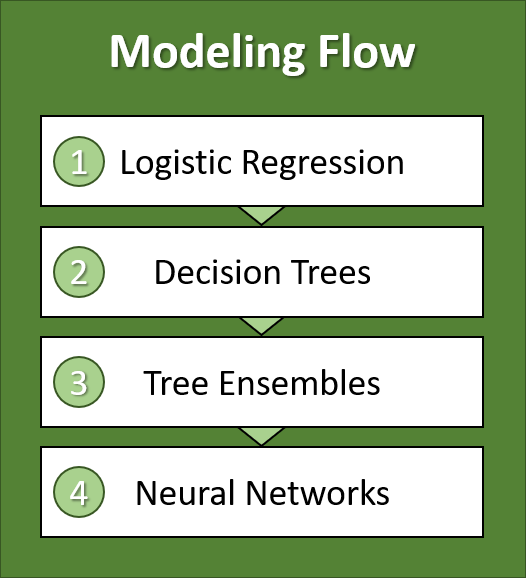
\includegraphics[width=.35\textwidth]{templates/images/Flow-Modeling.png}
\singlespacing
\caption[Machine learning modeling workflow]{Workflow for predicting the class of geothermal gradient in the Southwestern NM study area using a variety of common machine learning methods.}
\label{fig:model_flow}
\end{wrapfigure}

Supervised learning methods for classification come in a variety of shapes and sizes. Rather than settle on one for predicting geothermal gradient, four different methods are applied to the Southwestern NM data set. Figure \ref{fig:model_flow} illustrates the high-level modeling flow, where model complexity increases with successive steps. The method descriptions below only briefly delve into important model mechanics and key \textit{hyperparameters} (i.e., parameters not learned from data) that impact model performance. Other sources can provide a deeper review of machine learning algorithms and their mathematical underpinnings. This investigation should instead be considered an applied case study that uses these algorithms as tools for generating insights on geothermal potential.

\subsection{Assessing Performance}\label{ch3:modeling_assessments}
Building an intuition for the differences in predictive ability of various models first requires a clear definition of the scoring metric(s) used to compare those models. The characterization of classifier performance typically begins with a confusion matrix. In its simplest 2$\times$2 form, the confusion matrix evaluates binary class predictions as \acrlong{tp} (\acrshort{tp}; predicted 1, actually 1), \acrlong{tn} (\acrshort{tn}; predicted 0, actually 0), \acrlong{fp} (\acrshort{fp}; predicted 1, actually 0), and \acrlong{fn} (\acrshort{fn}; predicted 0, actually 1). For the multi-class problem, the confusion matrix expands to include all correct classification and misclassification options. Figure \ref{fig:confusion_matrix} illustrates the elements of a 4$\times$4 four-class matrix.

\begin{figure}[!htp]
\centering
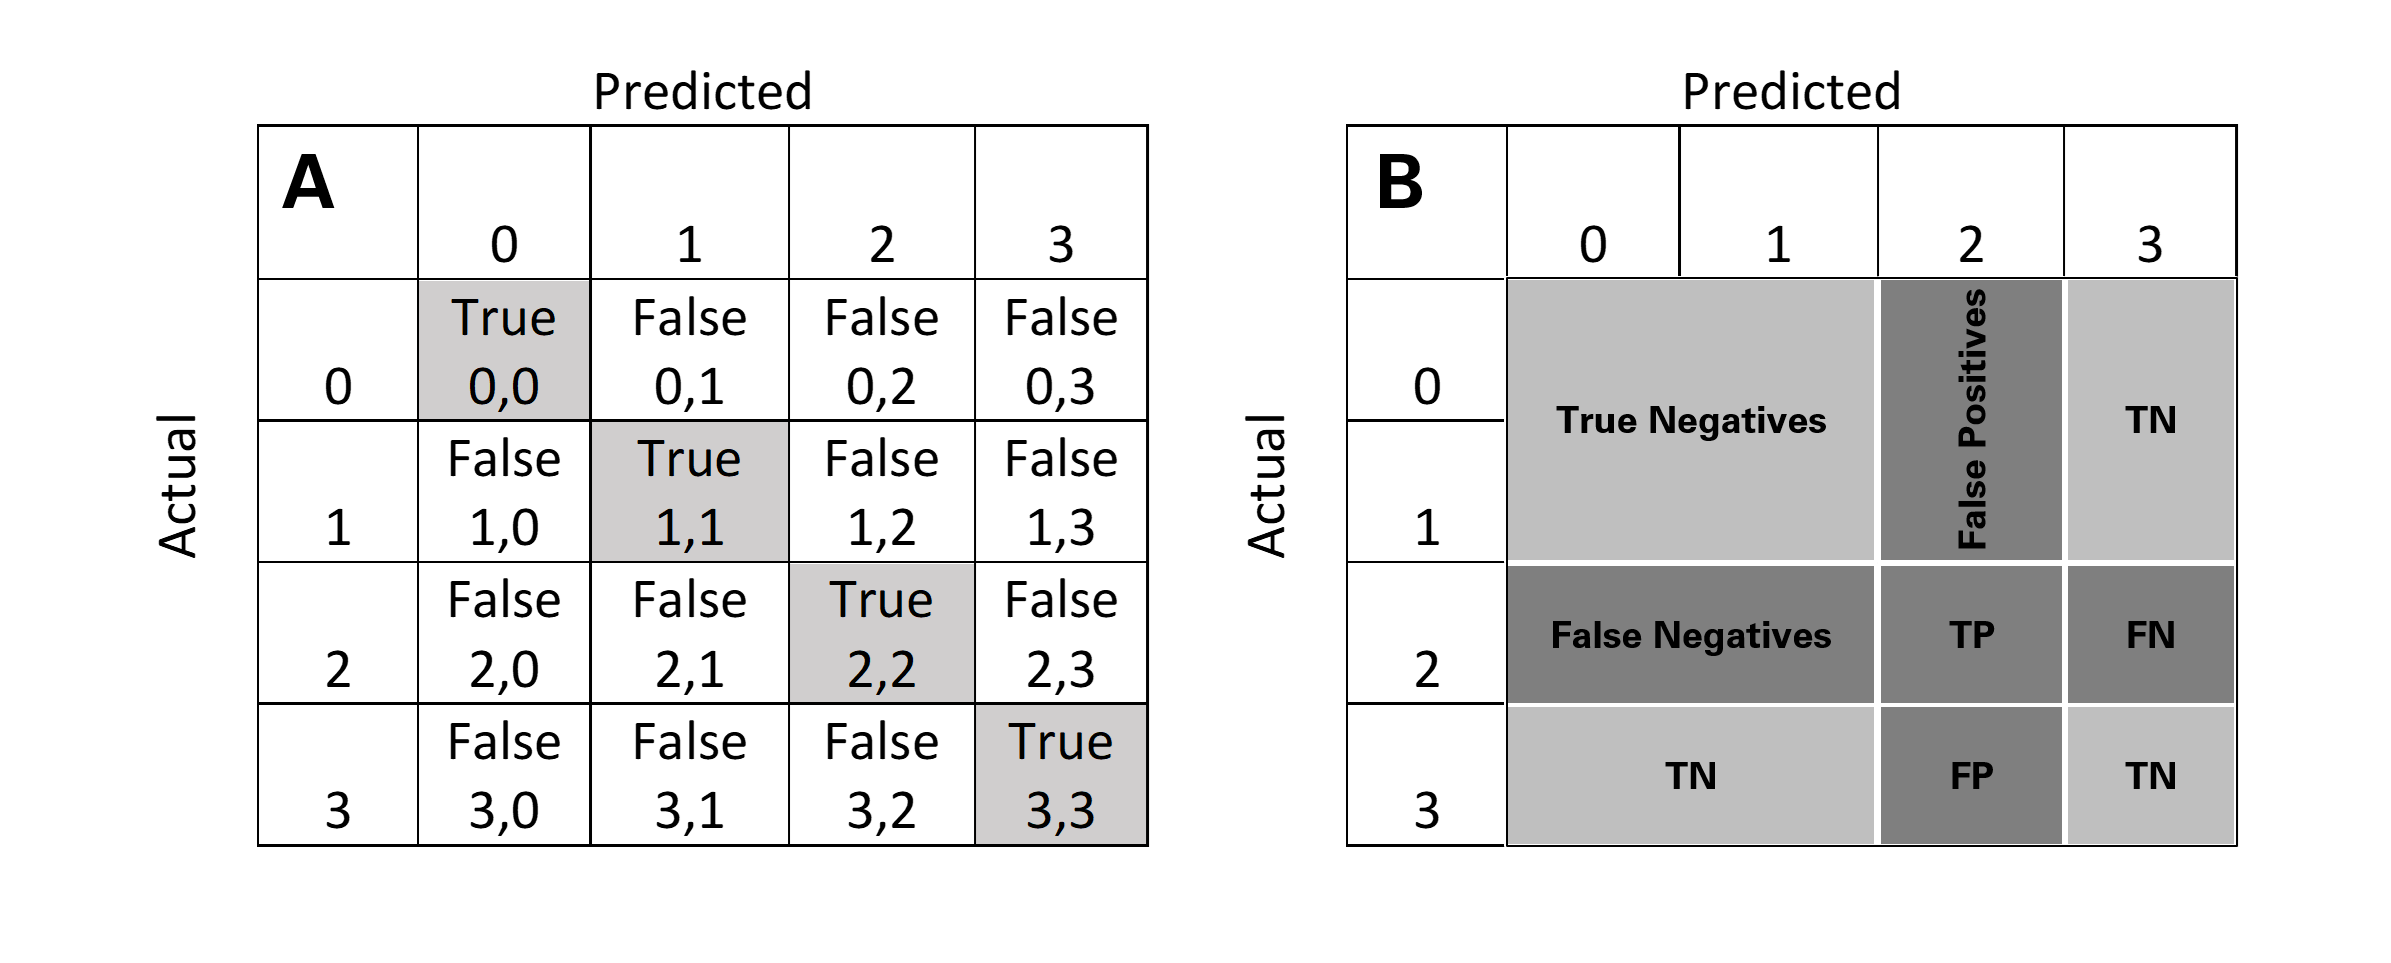
\includegraphics[width=\textwidth]{templates/images/Figure-Confusion_Matrix.png}
\caption[Example four-class confusion matrix]{Confusion matrix diagram for a 4-class scenario. A. Each cell represents a pairing between an actual class label (rows) and the predicted label (columns). True positives for each class are down the diagonal. B. Example of matrix interpretation using class 2 as a point of reference. Elements associated with TP, FP, TN, and FN values are labeled.}
\label{fig:confusion_matrix}
\end{figure}
Several statistical measures can be defined using combinations of elements in the confusion matrix. Of significance to this study are Accuracy, \acrlong{tpr} (\acrshort{tpr}) and \acrlong{fpr} (\acrshort{fpr}) \citep{tharwat_classification_2020}:

\begin{itemize}[itemsep=2pt]
\item \textbf{Accuracy}: the fraction of predictions that were correct:\\ (TP$+$TN)/(TP$+$TN$+$FP$+$FN)\\
\item \textbf{True Positive Rate}: the count of correctly-predicted positives scaled by the actual positives: TP/(TP$+$FN)
\item \textbf{False Positive Rate}: the count of incorrectly-predicted positives scaled by the actual negatives: FP/(FP$+$TN)
\end{itemize}

Classification relies on a probability threshold for assigning a class label. As the threshold lowers, the chance that the classifier believes it has a label match increases. By varying this threshold, it becomes possible to map out the discriminating ability of a classifier by plotting a curve in TPR vs. FPR space (Figure \ref{fig:roc}). This is commonly referred to as the \acrlong{roc} (\acrshort{roc}) curve \citep{fawcett_introduction_2006}. A classifier that cannot discriminate between classes performs no better than random guessing, with a curve that plots along the diagonal from the origin to the upper right of the plot. On the other hand, a perfect classifier has a TPR of 1.0 for all thresholds, so it plots up along the y-axis and then horizontally along TPR = 1.0. Typical ROC curves appear in the upper-left space between these two extremes.

\begin{figure}[!htp]
\centering
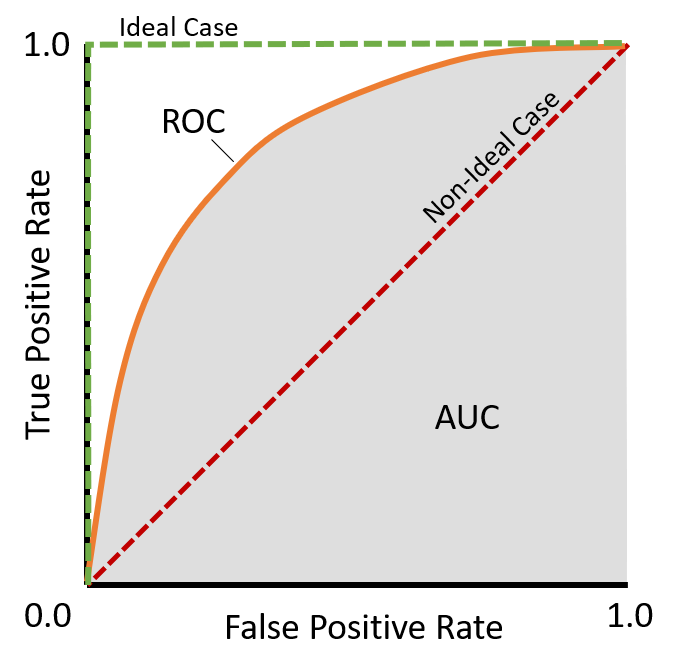
\includegraphics[width=0.5\textwidth]{templates/images/Figure-ROC_AUC_Diagram.png}
\caption[Receiver Operating Characteristic diagram]{ROC curve diagram in TPR vs. FPR space. Perfect classifiers will plot along the ideal case line (green), poor classifiers plot along the diagonal (red). AUC (gray) characterizes the quality of the classifier on a scale of 0.5 to 1.0.}
\label{fig:roc}
\end{figure}

Area Under the ROC Curve (AUC) defines a summary statistic for the ROC function (see Figure \ref{fig:roc}) \citep{fawcett_introduction_2006}. Since the ideal classifier has a TPR of 1.0 at all times, the ideal AUC also equals 1.0. In the non-ideal case, the AUC drops to 0.5. AUC values and ROC curves provide a standardized means of comparing classifiers and are the primary performance measures used in this thesis.

With multi-class classification, defining single class performance using the definitions of TP, FP, TN, and FN as shown in Figure \ref{fig:confusion_matrix}B is relatively straight-forward. Overall classifier performance across all classes can also be characterized with a single ROC curve using macro, weighted, or micro averaging \citep{scikit-learn_sklearnmetricsroc_auc_score_2021}.

\begin{itemize}[itemsep=2pt]
    \item \textbf{Macro averaging}: matches the unweighted arithmetic mean of metric values.
    \item \textbf{Weighted averaging}: follows the procedure of macro averaging but adds a weight for each class contribution based on the fraction of total observations that fall within that class. 
    \item \textbf{Micro averaging}: considers class results in aggregate, so statistics are calculated across the entire confusion matrix. TPR becomes the accuracy and FPR becomes the error rate.
\end{itemize}

For imbalanced data sets, a micro-average ROC curve will indicate better performance than the macro-average ROC curve due to the impact of the dominant class. Both micro- and macro-average ROC curves are included in the classification analysis for each machine learning model in this thesis.

\subsection{Hyperparameter Tuning}\label{ch3:strat_kfold_cv}
For a machine learning model to perform its best, the hyperparameters controlling model behavior must first be optimized or ``tuned.'' Assuming a large enough set of data is available, tuning simply involves training a series of classifiers with different values for a hyperparameter, assessing their performance against the validation data subset, and choosing the value with the best results. One statistically stable alternative approach useful for sparser data sets involves k-Fold \acrlong{cv} (\acrshort{cv}). By this method, the input data is split into k subsets, or folds. The model is repeatedly trained on the aggregate of all but one fold, then assessed against the remaining fold \citep[p. 181]{james_introduction_2013}. This leave-one-fold-out strategy cycles through all k permutations of splitting the data, and the scores are averaged to produce a summary statistic (e.g., AUC). For imbalanced class data, folds can be stratified-sampled such that class proportions of the unpartitioned data are preserved within each fold \citep{brownlee_how_2020}. 

When tuning a specific hyperparameter, the k-Fold CV process defines a set of average scores for the range of hyperparameter values under consideration, and the optimal parameter value can be determined from a plot of those scores. In some circumstances, a clear maximum in cross-validation results indicates the best value to use for modeling. In others, the CV curve levels off to form a corner or ``elbow.'' Choosing a hyperparameter value near this corner position balances the trade-off between overfitting and underfitting the training data.

\subsection{Logistic Regression}\label{ch3:logistic_regression}
\subsubsection{Algorithm Details} \label{ch3:lr_details}
The classic \acrlong{lr} (\acrshort{lr}) model is a binary classifier that predicts one of two labels based on the input data. Linear regression treats the problem as a linear combination of the input observations \citep[p.\ 369]{bertsimas_analytics_2016}:
\begin{equation}
\label{eq:linreg_form}
    \hat{y} = {\bf{w^Tx}} = w_0 + w_1 \cdot x_1 + w_2 \cdot x_2 + \ldots + w_n \cdot x_n 
\end{equation}
where $x_i$ are the feature observations, $w_i$ are coefficients or weights for those features, and $\hat{y}$ is the weighted sum. Logistic regression adjusts the problem such that predictions define the probability of belonging to class 1. This is done by using a non-linear logistic response function: 

\begin{equation}
\label{eq:sigmoid}
h_{\theta}(x) = \frac{1}{(1+e^{-\hat{y}})} = \frac{1}{(1+e^{-\textbf{w}^T\textbf{x}})}
\end{equation}

Equation \ref{eq:sigmoid}, also known as the \textit{sigmoid} function, converts the weighted sum from equation \ref{eq:linreg_form} to values between 0 and 1 \citep[p.\ 369]{bertsimas_analytics_2016}. Solving for the weights in this equation ($w_i$) requires an iterative optimization procedure like gradient descent. This procedure minimizes a cost function ($J(\Theta)$) based on the negative log likelihood \citep{ng_logistic_2011}:

\begin{equation}
\label{eq:logreg_cost}
\begin{aligned}
        J(\Theta) &= -\frac{1}{m} \sum_{i=1}^{m}{\text{Cost}(h_{\theta}(x_i),y_i)} \\ &= -\frac{1}{m}\sum_{i=1}^{m}{(y_i*\text{log}({h_{\theta}(x_i)})+(1-y_i)*\text{log}(1-h_{\theta}(x_i)))}
\end{aligned}
\end{equation}

Regularization is added to logistic regression to avoid overfitting, specifically by penalizing the sum of the squared weights (L2-regularization). A constant ($\lambda$) determines the trade-off of influence between the magnitude of the weights and negative log likelihood in the minimization \citep{ng_regularization_2011}.

\begin{equation}
\label{eq:logreg_cost_reg}
    regularized\,J(\Theta) = -\frac{1}{m}\sum_{i=1}^{m}{\text{Cost}(h_{\theta}(x_i),y_i) + \frac{\lambda}{2m}\sum_{j=1}^{n}{w_j^2}}
\end{equation}

The scikit-learn \textit{LogisticRegression} function used in this thesis applies a hyperparameter \verb|C| to the negative log likelihood term, which acts like the inverse of $\lambda$. Larger values of \verb|C| result in less regularization \citep{scikit-learn_logistic_2021}.

\subsubsection{Multi-Class Heuristics} \label{ch3:lr_multiclass}
The formulation of logistic regression defines a strictly binary classification problem without multi-class support. Two heuristic methods allow LR to extend to multi-class classification: \acrlong{ovo} (\acrshort{ovo}) and \acrlong{ovr} (\acrshort{ovr}) \citep{brownlee_one-vs-rest_2020,scikit-learn_multiclass_2021}. Both split the problem into multiple binary classifications. OvO considers every class versus every other class. In the 4-class geothermal gradient problem, this amounts to six classifications: {(0 vs. 1), (0 vs. 2), (0 vs. 3), (1 vs. 2), (1 vs. 3), (2 vs. 3)}. OvR simplifies the problem by combining class alternatives so the number of classifiers matches the number of classes: {(0 vs. [1, 2, or 3]),(1 vs. [0, 2, or 3]), (2 vs. [0, 1, or 3]),(3 vs. [0, 1, or 2])}. For both methods, the class with the greatest score or sum of scores wins, where the score is akin to the probability of class membership. This thesis uses the OvR strategy.

\subsubsection{Recursive Feature Selection} \label{ch3:lr_rfe}
By consequence of Equation \ref{eq:sigmoid}, logistic regression assumes a linear relationship between the weighted sum of independent predictors and the log-odds, i.e., $\log(\frac{P(y=1)}{1-P(y=1)})$. However, including all possible predictors will not necessarily improve the model. Feature selection can lead to simpler models with the same predictive power but reduced risk of collinearity, which is important when managing data from naturally-integrated earth systems.

One method for selecting the features to keep involves an iterative process called \acrlong{rfe} (\acrshort{rfe}) (Brownlee, 2020c; scikit-learn, 2021d). The concept is relatively simple: RFE recursively selects and removes the feature with the smallest coefficient in the logistic regression model, then refits the model to the data and repeats until a user-defined number of features is reached.  A plot of AUC vs. number of features can be constructed by looping over different feature limits, where the logistic regression model is fit on the training subset and evaluated on the validation subset. Much like in the CV process, the maximum will define the optimal number of features, and the elbow provides guidance when results show no clear maximum.

\subsection{Decision Trees}\label{ch3:decision_trees}
A decision tree, sometimes known as a Classification and Regression Tree (CART), classifies observations using a cascading set of evaluations, each on individual predictor variables. There is no assumption of a linear response in the system. In fact, decision trees are uniquely suited to representing non-linear behavior in a highly-explainable way; once constructed, the decision tree describes a flowchart-like road-map for each label assignment \citep[p. 373--375]{bertsimas_analytics_2016}. Not every predictor needs to appear in the decision tree, just those found to be significant during tree construction. And the most significant variables tend to be associated with early decision splits, placing them higher in the tree \citep[p. 376]{bertsimas_analytics_2016}. Because of this, decision trees naturally provide insights into feature importance. 

\subsubsection{Algorithm Details}\label{ch3:dtree_details}
Decision trees are constructed by recursively performing binary splits on the training data set. Each split defines two new nodes in the tree, which correspondingly partitions a group within the training data into two subgroups. These subgroups represent new terminal leaf nodes on the decision tree. The classification decision for each leaf will be the most commonly occurring class from the training data observations that are assigned to that leaf \citep[p. 311]{james_introduction_2013}.

There are three metrics that can play a role in evaluating the quality of a node in the decision tree:

\begin{itemize}[itemsep=2pt]\label{ch3:impurity}
    \item \textbf{Classification error rate}: the proportion of training samples that don't match the dominant class in a leaf node \citep[p. 312]{james_introduction_2013}.
    \begin{equation}
    \label{eq:error_rate}
        E = 1 - \max_k(\hat{p}_{mk})
    \end{equation}
    where $m$ is the subset of the data associated with a node, $k$ is the class, and $\hat{p}_{mk}$ is the fraction of all training observations in $m$ that are of class $k$. 
    \item \textbf{Gini index}: measures variance across all k classes. Gini is sometimes known as a purity measurement because low values correspond with a strongly dominant class \citep[p. 312]{james_introduction_2013}.
    \begin{equation}
    \label{eq:gini}
        G = \sum_{k=1}^{K}{\hat{p}_{mk}(1-\hat{p}_{mk})}
    \end{equation}
    \item \textbf{Entropy}: an alternative form of purity measure, which also shows low values when the proportion of one class dominates the others within a node \citep[p. 312]{james_introduction_2013}.
    
    \begin{equation}
    \label{eq:entropy}
        D = -\sum_{k=1}^{K}{\hat{p}_{mk}* \text{log}(\hat{p}_{mk})}
    \end{equation}
\end{itemize}

Tree construction takes place in two passes. In the forward pass, the tree will iteratively grow by selecting nodes in the tree, a predictor to split on, and a threshold value defining the split. These choices are made to maximize the purity of the child nodes, typically by using Gini index or entropy \citep[p. 307]{james_introduction_2013}. The tree will grow until a stopping condition is met, like reaching a maximum tree depth or minimum number of observations allowed per node. Tree clean-up or ``pruning'' then takes place in a backward pass, where the following decision tree objective governs whether a tree branch is kept or removed \citep[p. 309]{james_introduction_2013}:

\begin{equation}
\label{dtree_objective}
\begin{aligned}
    J(\Theta) &= E + \alpha\left|T\right| \\
    &= \left(1 - \max_k(\hat{p}_{mk})\right)+\alpha\left|T\right|
\end{aligned}
\end{equation}
\\
where $\left|T\right|$ refers to the number of terminal nodes in tree $T$ and the classification error rate ($E$) is used for measuring quality. The objective could rely on Gini index or entropy as well, but classification error rate will maximize prediction accuracy \citep[p.\ 312]{james_introduction_2013}. If $E$ increases by less than $\alpha$ when a branch is removed, that branch will remain removed from the decision tree. $\alpha$ acts as a regularization parameter balancing prediction accuracy with model complexity; greater values of $\alpha$ result in simpler decision trees.

\subsection{Tree Ensembles (XGBoost)}\label{ch3:tree_ensembles}
As simple and effective as decision tree classifiers may be, they only demonstrate a single model solution. And since random selection can play a role in their construction (e.g., in the scikit-learn implementation), a different tree structure may arise if the tree is rebuilt on the same data set. The random forest algorithm embraces these random variations and generates a large number of decision trees. To increase randomness, only a subset of the predictors are used when building each tree, and trees are trained on a data subset selected at random with replacement from the full training set \citep[p. 376--377]{bertsimas_analytics_2016}. Much like the classic ``wisdom of crowds'' paradigm, the collection of trees acts as a single, more performant ensemble model. However, greater potential accuracy in predictions trades off with less interpretability; as the forest grows larger, the number of constituent decision trees quickly exceeds the limits of human comprehension. As such, ensemble tree methods like random forests are considered black box algorithms.

\subsubsection{Algorithm Details}\label{ch3:xgb_details}
A variation on this ensemble method uses ``gradient boosting,'' where the trees are chained in succession and train on the residual error of the preceding tree. The trees are weak learners that underfit the data, giving them low variance, but high bias. Yet when they connect together through residual prediction, the final boosted model (Equation \ref{eq:xgb_form}) can out-perform conventional random forests \citep[p. 323]{james_introduction_2013}.

\begin{equation}
\label{eq:xgb_form}
    \hat{f}(x) = \sum_{b=1}^{B}{\alpha \hat{f}^{b}(x)}
\end{equation}
\\
where $\hat{f}(x)$ is the boosted model, $\hat{f}^b$ are the weak learners totaling $B$ in number, and $\alpha$ is the learning rate or shrinkage parameter. 

XGBoost, a variant of gradient-boosting tree algorithms, has gained notoriety from a history of machine learning competition wins \citep{chen_dmlcxgboost_2021}. The objective function governing XGBoost model construction balances two influences \citep{chen_xgboost_2016}:
\begin{equation}
\label{eq:xgb_objective}
\begin{aligned}
    J(\Theta) &= L + \Omega \\
    &= \sum_{i}{l(\hat{y}_i,y_i)}+\sum_{k}{\Omega(f_k)} \\
    &= \sum_{i}{l(\hat{y}_i,y_i)}+\sum_{k}{\left({\gamma T}+\frac{1}{2} \lambda \sum_{j=1}^T{w_j^2}\right)}
\end{aligned}
\end{equation}
\\
where the first part ($L$) expresses how well the model fits the data (i.e., the loss), while the second term ($\Omega$) regulates the complexity of the model. Complexity is defined by the number of leaves in a tree ($T$) and the size of leaf weights ($w$) that are unique to XGBoost decision trees. After some additional derivations, the objective can be restated as:

\begin{equation}
\label{eq:xgb_obj_simple}
    J(\Theta) = -\frac{1}{2}\sum_{j\;leaves}{\frac{G_j^2}{H_j + \lambda} + \gamma T}
\end{equation}
\\
where $G$ is the sum of the first-order gradient statistics for the instance set of leaf $j$, and $H$ is the sum of the second-order gradient statistics \citep{chen_xgboost_2016}. Tree construction follows that of decision trees --- split each node greedily to maximize tree depth, then prune back in a backward pass. The left term of Equation \ref{eq:xgb_obj_simple} provides a means to calculate loss reduction for a candidate split, thus governing the evaluation of tree splits during the pruning process. XGBoost is clearly a complex algorithm, but it comes with many optimizations that make it extremely efficient, scalable, and popular among machine learning practitioners.

\subsubsection{Shapley Analysis}\label{ch3:xgb_shapley}
Being a tree-based machine learning method, XGBoost naturally provides feature importances as a product of model-fitting. In fact, the XGBoost package offers five kinds of global feature importance calculations \citep{xgboost_developers_xgboost_2020}, but each can give slightly different results in feature ordering or relative feature impact on model predictive behavior. At issue here are two concepts in importance definition of ``feature attribution'' methods: \textit{consistency}, or the independence of a feature importance value and the reliance of a model on that feature, and \textit{local accuracy}, or the idea that the sum of the importances is equivalent to overall model importance \citep{lundberg_interpretable_2020}. A study of six different approaches to interpreting models through feature attribution showed only one method meets both of these properties: \acrlong{shap} (\acrshort{shap}) \citep{lundberg_consistent_2019}.

Shapley values derive from cooperative gain theory \citep{shapley_value_1997}, but have gained traction in the machine learning community partly because they predict importances without assuming complete feature independence \citep{lundberg_unified_2017}. In addition to managing collinearity, Shapley values have several desirable attributes. For example, if two features impact a model prediction equally, they will have equivalent Shapley values. And a Shapley value of zero means the feature has no predictive impact. The SHAP method produces values that have global significance for general feature importance but also local significance for an individual prediction; the sum of SHAP values is equivalent to the deviation of the model prediction from the average value (baseline), meaning SHAP values describe the individual feature contributions to a prediction value \citep{lundberg_unified_2017}. This thesis uses Shapley values directly provided by the XGBoost package \citep{xgboost_developers_xgboost_2020} for evaluating importances and for feature selection.

\subsection{Neural Networks}\label{ch3:ann}
The original concepts behind Artificial Neural Networks (ANNs or just \acrshort{nn}s) come from simplified models of neuron activity in the brain \citep[p.\ 394]{hastie_elements_2009}. At a high level, multiple inputs are fed into neuron cells from many branches on one end, and given the right combination of those inputs, these cells will fire and propagate a signal to the next group of connected neurons.
\begin{figure}[H]
\centering
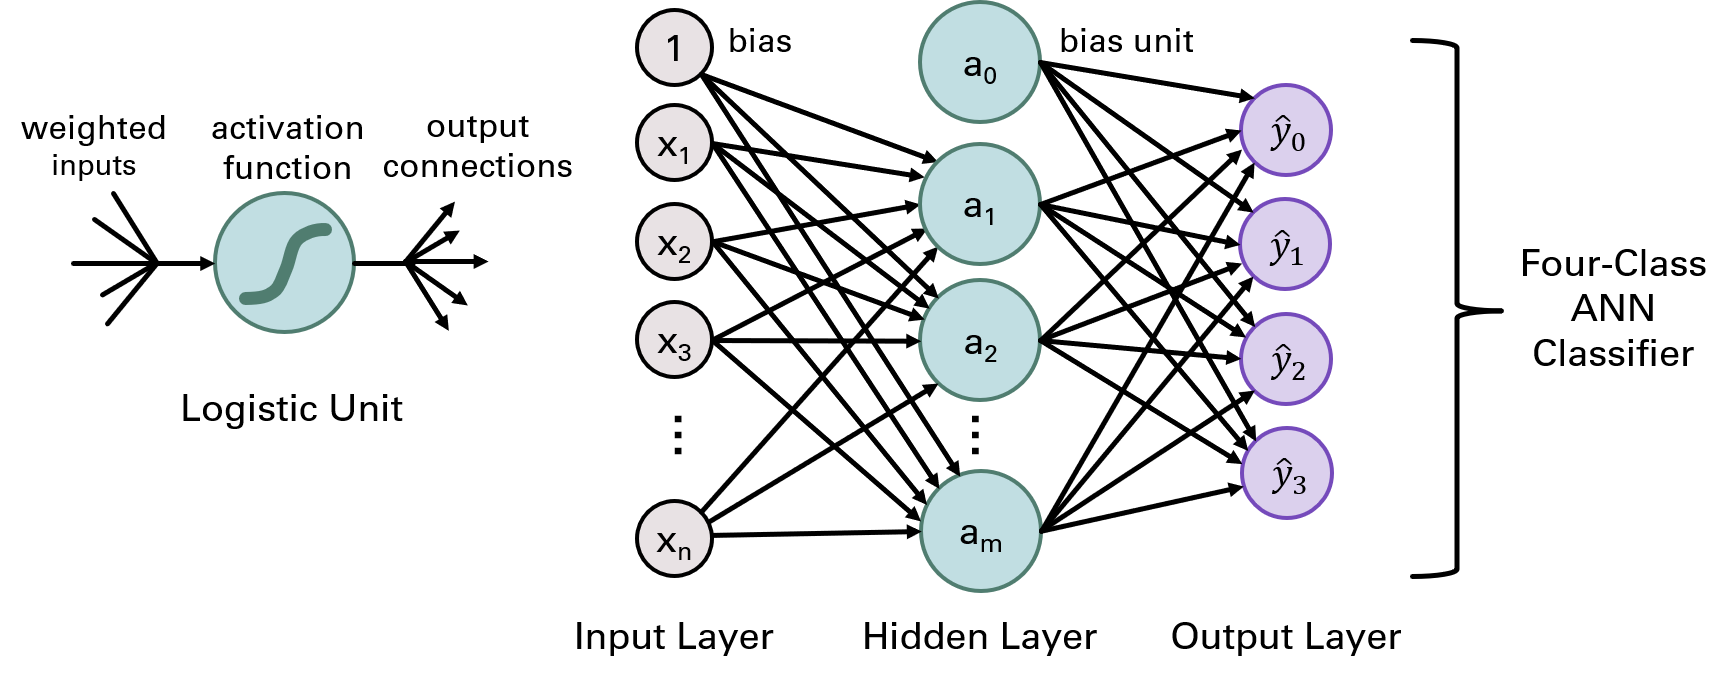
\includegraphics[width=\textwidth]{templates/images/Figure-ANN_schematic.png}
\caption[Neural network schematic]{Schematic of a logistic unit (Left) and a fully-connected neural network (Right) with a single hidden layer made up of logistic units $a_1$ through $a_m$. Bias units (subscript 0) traditionally have a value of 1, but are weighted in linear combinations like other units. Four units in the output layer make this a four-class classifier.}
\label{fig:nn_schematic}
\end{figure}

In neural networks, cells are represented by logistic units (Figure \ref{fig:nn_schematic}). Each unit acts like a logistic regression operation, where inputs are scaled by weights, and the linear sum of the weighted inputs are passed through an \textit{activation function} to determine if the output is a 0 or a 1. As in logistic regression, the sigmoid function (Equation \ref{eq:sigmoid}) appears in many network architectures, but other activation functions like the \acrlong{relu} (\acrshort{relu}) are common as well \citep{brownlee_gentle_2019}.

\subsubsection{Algorithm Details} \label{ch3:ann_details}
Each logistic unit performs the following operation:
\\
\begin{equation}
\label{eq:nn_activation}
    {\bf{a}} = g({\bf{z}}) = g({\bf{W^TX}})
\end{equation}
\\
where $g$ is the activation function and $\bf{W}$ is a matrix of weights. For the first hidden layer, $\bf{X}$ will be the predictor values from the input layer as shown in Figure \ref{fig:nn_schematic}. For any additional hidden layers, $\bf{X}$ consists of the outputs of units from the preceding layer. $\bf{z}$ is analogous to \(\hat{y}\) in Equation \ref{eq:linreg_form}.

The cost function for a neural network takes on the form of a loss term and a complexity term \citep{ng_neural_2011}:
\begin{equation}
\label{eq:nn_cost_function}
    \begin{aligned}
        J(\Theta) &= 
        -\frac{1}{m}\sum_{i=1}^{m}{
        L(\hat{y}_i, y_i)} + \frac{\lambda}{2m}
        \sum_{l=1}^{L-1}{
        \sum_{i=1}^{s_l}{
        \sum_{j=1}^{s_{l+1}}{(w_{ij}^{l})^2}}} \\
        &= -\frac{1}{m}
        \sum_{i=1}^{m}{
        \sum_{k=1}^{K}{
        y_k^{(i)}\log{h_{\theta}(x^{(i)})_k}+
        (1-y_k^{(i)})\log{(1-h_{\theta}(x^{(i)})_k)}}}\ + \\
        &\qquad \frac{\lambda}{2m}
        \sum_{l=1}^{L-1}{
        \sum_{i=1}^{s_l}{
        \sum_{j=1}^{s_{l+1}}{(w_{ij}^{l})^2}}}
    \end{aligned}
\end{equation}
\\
Note the similarity in appearance to the regularized negative log likelihood cost function for logistic regression (Equation \ref{eq:logreg_cost_reg}). Here, $m$ is the number of predictor values in the input layer, $K$ is the number of outputs, $L$ is the number of layers, and $i$ and $j$ track the weights for layer $j$, unit $i$. $\lambda$ is a regularization term controlling the balance between the loss term and complexity term in the cost function. Minimizing this cost function is the goal of the neural network training process. This is generally accomplished using the backpropagation algorithm to compute the gradients needed for a gradient descent optimization \citep[p.\ 396]{hastie_elements_2009}.

\section{Uncertainty Analysis}\label{ch3:uncertainty_analysis}
In the case study considered in this thesis, each of the four supervised machine learning methods discussed so far will generate different predictions for geothermal gradient at each point across the Southwestern NM AOI. But presenting these results to an explorationist will invariably elicit two important questions: 1) Which of these model results is the right one? and 2) What actions should I take based on these models? 

%\begin{wrapfigure}{R}{0.45\textwidth}
\begin{figure}[!htp]
\centering
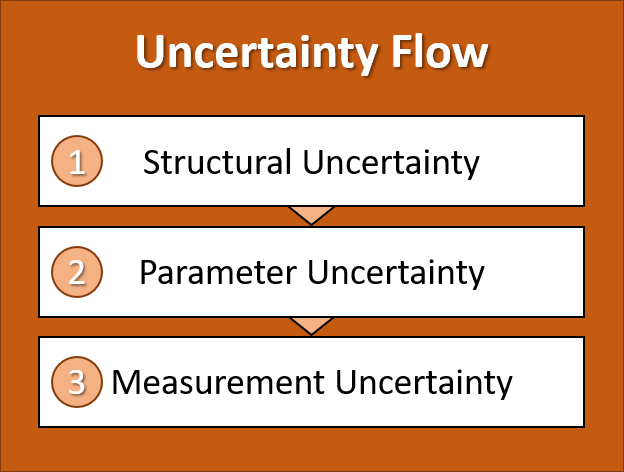
\includegraphics[width=.35\linewidth]{templates/images/Flow-Uncertainty.png}
\singlespacing
\caption[Uncertainty analysis workflow]{Workflow for analyzing uncertainties in model results for geothermal gradient prediction across the Southwestern NM study area.}
\label{fig:uncertainty_flow}
%\end{wrapfigure}
\end{figure}

George Box famously remarked, ``Essentially, all models are wrong, but some are useful'' \citep{box_empirical_1987}, which serves as an effective answer to the first question. But knowing that none of the prediction maps is individually correct falls short of providing impactful and actionable information for geothermal exploration decision-makers. Value lies in describing the sources of uncertainty and where those uncertainties manifest in a spatial prediction of geothermal gradient or other modeled risk elements. To this end, the following analysis considers uncertainties from the three sources described in Section \ref{ch2:uncertainty} and illustrated in Figure \ref{fig:uncertainty_flow}: model type (structural), model calibration (parameter), and model input (measurement).

\subsection{Classification Uncertainty Measures}\label{ch3:uncertainty_measures}
Unlike standard regression problems that result in continuous variable predictions, classifiers are inherently limited to selecting among $n$ discrete class values. Variability in model results cannot be measured by standard deviation. For geospatial classifications, the simplest comparison between maps is visual; plotting two displays side-by-side can effectively communicate qualitative differences. Quantifying the uncertainty of categorical predictions based on multiple realizations defines a more difficult problem, with a variety of different statistical approaches to consider. Among these are performance measures based on the class assignments, including percent correctly classified (accuracy), confusion matrix, AUC, Kappa \citep{cohen_coefficient_1960}, and weighted Tau \citep{ma_tau_1995}. Other methods consider the probabilities that precede the final classification choice, including Brier score \citep{brier_verification_1950} and Shannon entropy \citep{shannon_mathematical_1948}.

Rather than perform an exhaustive search through different metrics, this thesis follows the recommendation of \citep{beaudette_accuracy_2020} in characterizing classification uncertainty using entropy. Although the standard entropy calculation (Equation \ref{eq:entropy}) does not account for class similarity, it does show good discrimination ability for model results with low, medium, and high stand-out probability for the majority class \citep{beaudette_accuracy_2020}. A normalized version of the entropy calculation is as follows:
\begin{equation}
\label{eq:norm_entropy}
    H = -\frac{1}{\log_2{(n)}}\sum_{i=1}^{n}{p_i \cdot \log_2{(p_i)}} = -\sum_{i=1}^{n}{p_i \cdot \log_n{(p_i)}}
\end{equation}
\\
where $p_i$ represents the probability assigned to class label $i$. Entropy maps can be constructed with the output probabilities of a single classification model or from the results of an ensemble of model predictions by first averaging across class probabilities for all models at each map location.

\subsection{Structural Uncertainty}\label{ch3:structural_uncertainty}
The specific choice of classification algorithm implicitly applies constraints on the solution space for the problem. For example, logistic regression solutions assume there is a linear relationship between predictor variables and the log-odds of the response variable. And decision trees use hard thresholds that can create step-like model behavior. Model formulations thus influence the individual results and range of results that a model is capable of producing.

In order to examine the uncertainty introduced by structural aspects of the chosen machine learning models, the predicted class probabilities for multiple models can be averaged together to create an ensemble prediction of geothermal gradient classes. Shannon entropy can then be calculated for the class probabilities of this average model and displayed as a map, with normalized values between 0 to 1. High entropy locations mark regions where there is no clear differentiation between most-likely gradient class labels. Low entropy locations indicate the opposite --- multiple models agree on a single dominant class label for that area.

\subsection{Parameter Uncertainty}\label{ch3:param_uncertainty}
The fitting procedure for machine learning models generally involves minimizing a cost function as updates are iteratively made to model parameters, e.g., feature weights. However, the final trained models treat these parameters as deterministic values with no uncertainty. Using neural networks as an example, the complexity of the model architecture and the potential for different parameterizations as randomness in techniques like dropout and mini-batching influence the training process, suggest a deterministic view insufficiently represents the model space. By defining the range of uncertainty on model parameters, it is possible to generate many solutions from the same model --- an ensemble of valid predictions. Uncertainty estimates derived from this ensemble can introduce a measure of confidence in a model’s output, allowing the model to directly explain what it knows and, more importantly, what it doesn’t know in the solutions it produces.

The Google DeepMind team introduced a method called ``Bayes by Backprop'' in 2015 where single-value weights are replaced by probability distributions in a neural network architecture \citep{blundell_weight_2015}. Making the simplifying assumption that the weight distributions are Gaussian, each weight parameter in a standard ANN layer is replaced by a mean and a standard deviation in a probabilistic layer. A fully-trained \acrlong{bnn} (\acrshort{bnn}) samples from the weight distributions for just-in-time determination of weight values as data is fed through to produce a prediction. Therefore, each prediction of the BNN varies depending on the selected weights, and running the network many times on the same data set will produce a set of different results. An analysis of the variation in this solution ensemble can characterize how parameter uncertainty impacts BNN classification performance.

At a fundamental level, BNNs operate using Bayes theorem for training the network \citep{webster_probabilistic_2021}:

\begin{equation}
    \label{eq:bayesrule}
    P({\bf w} \vert D) = \frac{P(D \vert {\bf w}) \cdot P({\bf w})}{P(D)}
\end{equation}
\\
where ${\bf w}$ are the model weights and $D$ are the observed data. $P({\bf w})$ define the \textit{priors}, or the distributions assigned to the weights before seeing $D$. $P(D \vert {\bf w})$ defines the likelihood of $D$ given ${\bf w}$. $P({\bf w} \vert D)$ are the \textit{posteriors} or the distributions after taking $D$ into account.

In practice, BNNs use a Variational Bayes method, which approximates $P({\bf w} \vert D)$ with a variational posterior, $q({\bf w} \vert \theta)$. The desired difference between these two functions is zero (perfect approximation), so this defines the basis of a loss function measured using the Kullback-Leibler divergence \citep{webster_probabilistic_2021}:

\begin{equation}
    \label{eq:bnn_loss}
    \begin{aligned}
    D_{KL}\left(q({\bf w} \vert \theta)\ \vert\vert\ P({\bf w} \vert D)\right) &= \int{q({\bf w} \vert \theta) \log \left({\frac{q({\bf w} \vert \theta)}{P({\bf w} \vert D)}}\right) d{\bf w}} \\
    &= \log P(D) + D_{KL}\left(q({\bf w} \vert \theta)\ \vert\vert\ P({\bf w})\right) \\ 
    &\qquad- \mathbf{E}_{q({\bf w} \vert \theta)}\left[\log P(D \vert {\bf w})\right]
    \end{aligned}
\end{equation}
\\
Dropping constant terms and treating this as an objective to minimize \citep{blundell_weight_2015}:
\begin{equation}
    \label{eq:bnn_objective}
    J(\Theta) = D_{KL}\left(q({\bf w} \vert \theta)\ \vert\vert\ P({\bf w})\right) - \mathbf{E}_{q({\bf w} \vert \theta)}\left[\log P(D \vert {\bf w})\right]
\end{equation}

This two-term objective describes a trade-off between the complexity as controlled by deviation from the prior ($P({\bf w})$) and the negative log-likelihood term measuring the fit to the data.

In this thesis, the TensorFlow Probability package is used to transform the ANN from Section \ref{ch3:ann} into a BNN for uncertainty estimation \citep{dillon_tensorflow_2017}. Running a trained BNN multiple times will produce a collection of different results due to the randomness in the model. Geothermal gradient class probabilities from these realizations can be averaged by class for each point location, and entropy values calculated from the ensemble-averaged probabilities to examine parameter uncertainty.

\subsection{Measurement Uncertainty}\label{ch3:measure_uncertainty}
Data modeling and analytics generally begin with the collection, engineering, and conditioning of features of interest. Building the perfect dataframe for machine learning may be the first priority, but capturing standard error estimates for its constituent features is fundamental to understanding how much uncertainty they bring to the prediction problem.

With appropriate measures of standard error, the values for each feature in a data set can be perturbed to create a range of statistically-similar derivative data sets. Variability in the classifications from these data sets highlights model sensitivity to uncertainties in the feature measurements. As with the other uncertainties, the predicted class probabilities for model realizations using the different data sets can be ensemble-averaged at each point within the AOI. And summary statistics like Shannon entropy calculated from the class probabilities indicate where the predictive power of the model is most sensitive to measurement uncertainty. This procedure can apply to a single feature, group of features, or all features at once to reveal how individual features or combinations of features impact model uncertainty.
\vfill
\section{Recap}\label{ch3:recap}
This chapter discussed the data sources and conditioning steps followed to prepare a data set for exploration-scale predictive modeling of the Southwestern NM study area. Detailed information on each GIS data layer is presented in Appendix \ref{app:A_data_layers}. The machine learning models and uncertainties under consideration were also outlined. Key take-away messages from this chapter include the following:

\begin{enumerate}
    \item Data sets gathered from geothermal archives, academic and agency repositories, and directly from the literature require extensive preparation to create consistent GIS layers as input features for modeling.
    \item The predictor variables total 25 features that collectively measure aspects of the fluids, heat, and permeability geothermal risk elements.  The response variable, geothermal gradient, represents a proxy for the heat risk element and is binned into 4 ranges representing non-thermal, low-grade, mid-grade, and high-grade gradient values for prediction.
    \item Collinearity is an issue for several features. Average Air Temperature is very tightly coupled with Surface Topography and was preemptively removed from the set of predictors.
    \item The relatively sparse well data set (WDS) used to train the supervised machine learning models is augmented by creating adjacent pseudowells for each original well location. WDS4 adds pseudowells in the N, S, E, and W directions. WDS8 extends WDS4 with NE, SE, SW, and NW pseudowells.
    %\item Standard scaling and power transformations applied to the feature data result in feature distributions that are more standard normal in appearance. This conditioning helps improve performance and aligns with statistical assumptions of some algorithms.
    \item Data sets are split into training, validation, and testing subsets using a stratified sampling technique to preserve the distribution of geothermal gradient classes.
    %\item To prevent data leakage, scaling and transformation methods are tuned on the training subset alone before being applied to the validation and testing subsets.    
    \item Machine learning models investigated in this thesis include logistic regression, decision tree, tree-based ensemble (XGBoost), and a neural network.
    \item Assessments of classifier performance span multiple dimensions. Here, models are assessed and compared using confusion matrices, classifier accuracy, AUC, and ROC plots.
    %\item A k-fold Cross-Validation method for hyperparameter tuning manages the issue of sparse input data.
    \item Feature importances describe the relative influence different features have on the prediction from a classifier. Some models provide this directly, others require routines like RFE to rank the features.
    \item Structural uncertainty refers to classification uncertainty tied to model structure. This is evaluated both by visual results comparison and entropy calculations from an ensemble of model results.
    \item Parameter uncertainty refers to classification uncertainty from the model parameterization. This is examined through entropy analysis of a results ensemble generated using a Bayesian Neural Network.
    \item Measurement uncertainty refers to classification uncertainty related to the standard errors of input feature values. This is evaluated by generating statistically-similar variations of the input data and comparing model results through entropy analysis. 
\end{enumerate}

Results from applying these methods and models in the context of a risk-mitigation strategy for geothermal exploration are explored in Chapter \ref{ch5:ml_results}.